
% Hamzeh Khanpour
% Top FCNC search at FCC-ee
% From the FCC-ee precision programme to rare top interactions


\documentclass[aspectratio=1610,10pt,english]{beamer}

\usepackage{babel}
\usepackage[T1]{fontenc}
\usepackage[utf8]{inputenc}
\usepackage{lmodern}

\usepackage{amsmath,amssymb,bm}
\usepackage{array}
\usepackage{booktabs}
\usepackage{multirow}
\usepackage{graphicx}
\usepackage{ragged2e}
\usepackage{etoolbox}
\usepackage{tikz}
\usepackage{tabularx}
\usepackage{hyperref}
\usepackage{xcolor}
\usepackage{tcolorbox}

\usetikzlibrary{arrows.meta,decorations.markings,decorations.pathmorphing,calc}
\usetikzlibrary{positioning,shapes.geometric,fit}

\makeatletter
\patchcmd{\itemize}{\raggedright}{\justifying}{}{}
\patchcmd{\beamer@enum@}{\raggedright}{\justifying}{}{}
\patchcmd{\@@description}{\raggedright}{\justifying}{}{}
\makeatother

\mode<beamer>{
	\definecolor{links}{HTML}{2A1B81}
	\hypersetup{
		pdfpagemode=FullScreen,
		colorlinks=true,
		linkcolor=links,
		urlcolor=links,
		citecolor=links
	}
	\usetheme[parttitle=rightfooter]{AGH}
}


%\setbeamercolor{title in head/foot}{fg=white}
%\setbeamercolor{author in head/foot}{fg=white}
%\setbeamercolor{date in head/foot}{fg=white}
%\setbeamercolor{part title}{fg=white}


\graphicspath{
	{./}
	{Presentation_Higgs_performance_meeting19marc_2024/}
	{Presentation_Higgs_performance_meeting19marc_2024/240GeV-leptonic/}
	{Presentation_Higgs_performance_meeting19marc_2024/240GeV-fullhadonic/}
	{Presentation_Higgs_performance_meeting19marc_2024/365GeV-leptonic/}
	{Presentation_Higgs_performance_meeting19marc_2024/365GeV-fullhadronic/}
	{Presentation_Higgs_performance_meeting19marc_2024/Plots-240/}
	{Presentation_Higgs_performance_meeting19marc_2024/Plots-365/}
	{top_FCNC_FCCee_draft/}
	{top_FCNC_FCCee_draft/images/}
	{top_FCNC_FCCee_draft/Jet-Algorithm/}
	{top_FCNC_FCCee_draft/240GeV-leptonic/}
	{top_FCNC_FCCee_draft/240GeV-fullhadonic/}
	{top_FCNC_FCCee_draft/365GeV-leptonic/}
	{top_FCNC_FCCee_draft/365GeV-fullhadronic/}
	{PresentationKrakow_2023/}
{Figs/}
{arXiv-2505.00272v1/Physics/Overview/Figs/}
{arXiv-2505.00272v1/Physics/PhysicsCase/Figs/}
{arXiv-2505.00272v1/Physics/DetectorRequirements/Figs/}
{arXiv-2505.00272v1/Physics/DetectorConcepts/Figs/}
}

\setbeamertemplate{navigation symbols}{}
\setlength{\tabcolsep}{4pt}
\renewcommand{\arraystretch}{1.15}

\newcommand{\placeholdergraphic}[2]{%
	\begin{center}
		\setlength{\fboxsep}{6pt}%
		\fbox{%
			\begin{minipage}[c][#2][c]{0.94\linewidth}
				\centering\textbf{Placeholder for official screenshot}\\[0.5ex]
				\footnotesize #1
		\end{minipage}}
	\end{center}
}

\newcommand{\refs}[1]{\vspace{0.35em}{\raggedleft\scriptsize\color{gray}Refs: #1\par}}
\newcommand{\takehome}[1]{\begin{alertblock}{Take-home message}\small #1\end{alertblock}}
\newcommand{\smaller}[1]{{\fontsize{8}{9.3}\selectfont #1}}
\newcommand{\tinyref}[1]{{\raggedleft\tiny\color{gray}#1\par}}

\title[{\color{white}Top FCNC search at the FCC-ee}]{{\color{white}Top FCNC search at the FCC-ee}}
\subtitle{From the FCC-ee precision programme to rare top interactions}
\author[Hamzeh Khanpour]{Hamzeh Khanpour}
\institute[AGH]{Faculty of Physics and Applied Computer Science\\AGH University of Krakow}


\date[Seminarium HEP Białasówk]{%
  \begingroup
\setlength{\fboxsep}{5pt}%
\fcolorbox{red!70!black}{green!12}{%
\parbox{0.50\linewidth}{\centering
Seminarium HEP Białasówk; 15 May 2026}
}%
  \endgroup
}


\begin{document}



%----------------------------------------------------------------------------------------
\begin{frame}[plain]
		
\begin{tikzpicture}[remember picture,overlay]
\node[
anchor=north east,
xshift=-0.55cm,
yshift=-0.95cm
] at (current page.north east)
{
\includegraphics[width=3.05cm]{FCC.jpg}};
\end{tikzpicture}
		
\titlepage
		

\end{frame}
%----------------------------------------------------------------------------------------
	
	
	
	
	
%----------------------------------------------------------------------------------------
\begin{frame}{FCC-ee feasibility studies from our group}
\begin{tcolorbox}[colback=white,colframe=blue!85!black,boxrule=0.8pt,arc=2mm]
\small
\justifying 
\textbf{Bottom quark forward-backward asymmetry at the future electron-positron collider {\color{magenta}FCC-ee}}\\
Marina Cobal (Udine U.), Giovanni Guerrieri (Udine U.), Hamzeh Khanpour ({\color{magenta}AGH}), Giancarlo Panizzo (Udine U.), Michele Pinamonti (ICTP), Laura Pintucci (ICTP), Leonardo Toffolin (University of Trieste)\\
{\color{blue}To evaluate how FCC-ee can clarify the long-standing $A_{FB}^{0,b}$ anomaly with the huge Z-pole data sample and much improved precision.}
\end{tcolorbox}
\vspace{-0.1cm}
\refs{{\color{red}$A_{FB}^{0,b}${\color{blue}@}FCC-ee analysis note: FCC Physics and Experiments:  https://repository.cern/records/g97j3-q0w73}.}


\vspace{0.3cm}


\begin{tcolorbox}[colback=white,colframe=red!85!black,boxrule=0.8pt,arc=2mm]
\small
\justifying 
\textbf{Top quark FCNC anomalous couplings at the future collider {\color{magenta}FCC-ee}}\\
Patrizia Azzi (INFN Padova), Hamzeh Khanpour ({\color{magenta}AGH}), Mojtaba Mohammadi Najafabadi (CERN), Emmanuel Francois Perez (CERN), Seddigheh Tizchang (IPM)\\
{\color{blue}To determine the FCC-ee reach for rare top-FCNC interactions, especially $tq\gamma$ and $tqZ$, in single-top production.}
\end{tcolorbox}
\vspace{-0.1cm}
\refs{{\color{red}Top FCNC analysis note: FCC Physics and Experiments:  https://repository.cern/records/avxy7-mtz86}.}



\begin{tikzpicture}[remember picture,overlay]
\node[
anchor=north east,
xshift=-0.1cm,
yshift=-0.3cm
] at (current page.north east)
{
\includegraphics[width=1.8cm]{FCC.jpg}};
\end{tikzpicture}


\end{frame}







%----------------------------------------------------------------------------------------
\section{{\color{white}FCC programme and physics motivation}}



\begin{frame}{Why a future collider programme after the LHC?}
\begin{itemize}
\justifying
\item The LHC has completed the Standard-Model particle spectrum, but not the \alert{origin of electroweak symmetry breaking}, the flavor puzzle, or the scale of new dynamics.
\item If new physics is heavy or weakly coupled, the most sensitive handles can be \alert{precision measurements} and \alert{rare\&forbidden processes} rather than direct production.
\item A next collider programme therefore needs both: \textbf{({\color{magenta}i})} a precision stage to expose small deviations and \textbf{({\color{magenta}ii})} an energy-frontier stage to map the underlying dynamics.
\item This is exactly the logic of the integrated FCC programme: exploit the clean \(e^+e^-\) environment first, then extend to the 100~TeV hadron frontier.
\end{itemize}


%\begin{alertblock}{Physics angle for this talk}
%\justifying
%\small Top FCNC is a textbook example of a \emph{rare, symmetry-suppressed observable} whose discovery potential is magnified by a precision \(e^+e^-\) environment.
%\end{alertblock}



\begin{exampleblock}{Key official FCC sources}
\justifying
\small
{\color{magenta}FCC Feasibility Study Report}: Physics, Experiments, Detectors,
{\color{blue}Eur.~Phys.~J.~C 85 (2025) 1468}. \\
{\color{magenta}FCC Physics Opportunities, FCC CDR}: physics case and benchmark programme,
{\color{blue}Eur.~Phys.~J.~C 79 (2019) 474}. \\
{\color{magenta}Physics Briefing Book}: Input for the 2026 update of the European Strategy for Particle Physics,
{\color{blue}2511.03883 [hep-ex]}. 
\end{exampleblock}



\begin{tikzpicture}[remember picture,overlay]
\node[
anchor=north east,
xshift=-0.1cm,
yshift=-0.3cm
] at (current page.north east)
{
\includegraphics[width=1.8cm]{FCC.jpg}};
\end{tikzpicture}



\end{frame}






%----------------------------------------------------------------------------------------
\begin{frame}{The FCC integrated vision: FCC-ee to FCC-hh}
\begin{columns}[T]%[T,totalwidth=\textwidth]
	
\begin{column}{0.58\textwidth}
	
\begin{itemize}
\justifying
\item {\color{magenta}Stage 1:} FCC-ee: high-luminosity precision programme from the $Z$ pole to the top threshold.
\item {\color{magenta}Stage 2:} FCC-hh: $\sim 100~\mathrm{TeV}$ proton-proton collider in the same civil infrastructure.
\item The strength of the programme is {\color{blue}complementarity}: absolute precision first, direct reach afterwards.
\item FCC-ee provides clean reference measurements of Higgs couplings, EW observables and top properties that sharpen the FCC-hh physics interpretation.
\end{itemize}

\end{column}

\begin{column}{0.50\textwidth} 
\centering
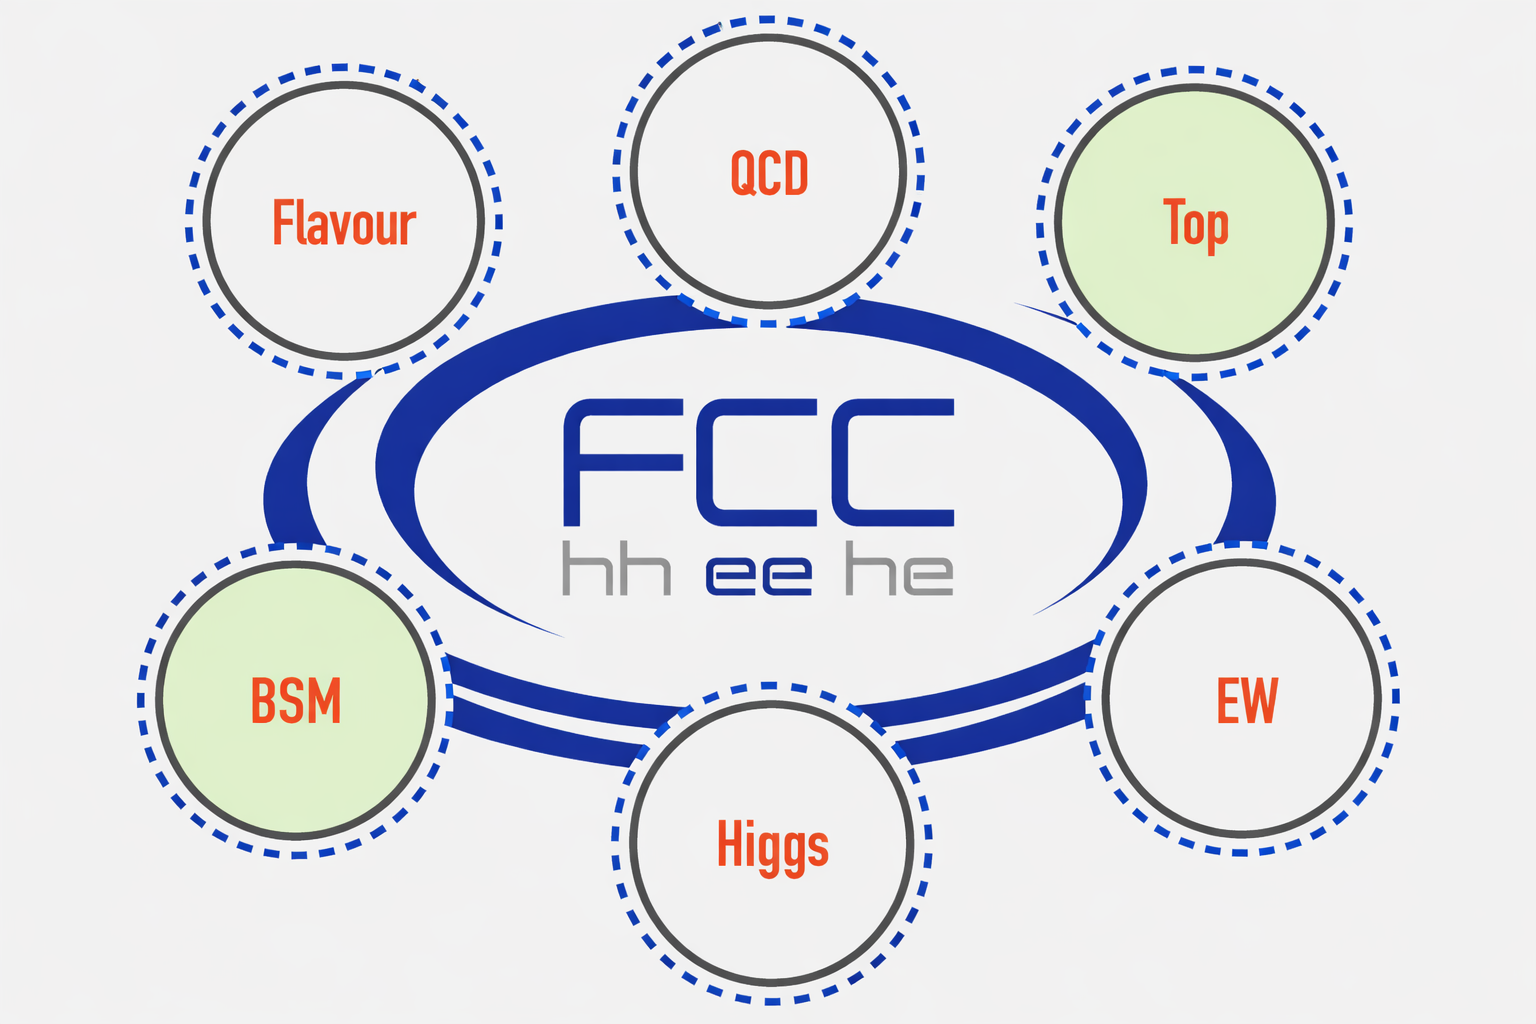
\includegraphics[width=\linewidth]{FCC_ee_1.png} 
\end{column} 
\end{columns} 

\takehome{ 
\justifying
\small
FCC-ee would establish the precision reference frame of the programme: per-mille-level Higgs normalisation, ultra-precise $Z/W$ observables, and threshold top measurements. FCC-hh then uses this foundation to explore rare Higgs processes, the Higgs self-coupling and direct high-mass new physics.} 


\begin{tikzpicture}[remember picture,overlay]
\node[
anchor=north east,
xshift=-0.1cm,
yshift=-0.3cm
] at (current page.north east)
{
\includegraphics[width=1.8cm]{FCC.jpg}};
\end{tikzpicture}


\end{frame}







%----------------------------------------------------------------------------------------
\begin{frame}{FCC-ee running points: one collider, several precision laboratories}
\small
\begin{columns}[T]%[T,totalwidth=\textwidth]
\begin{column}{0.50\textwidth}
\centering
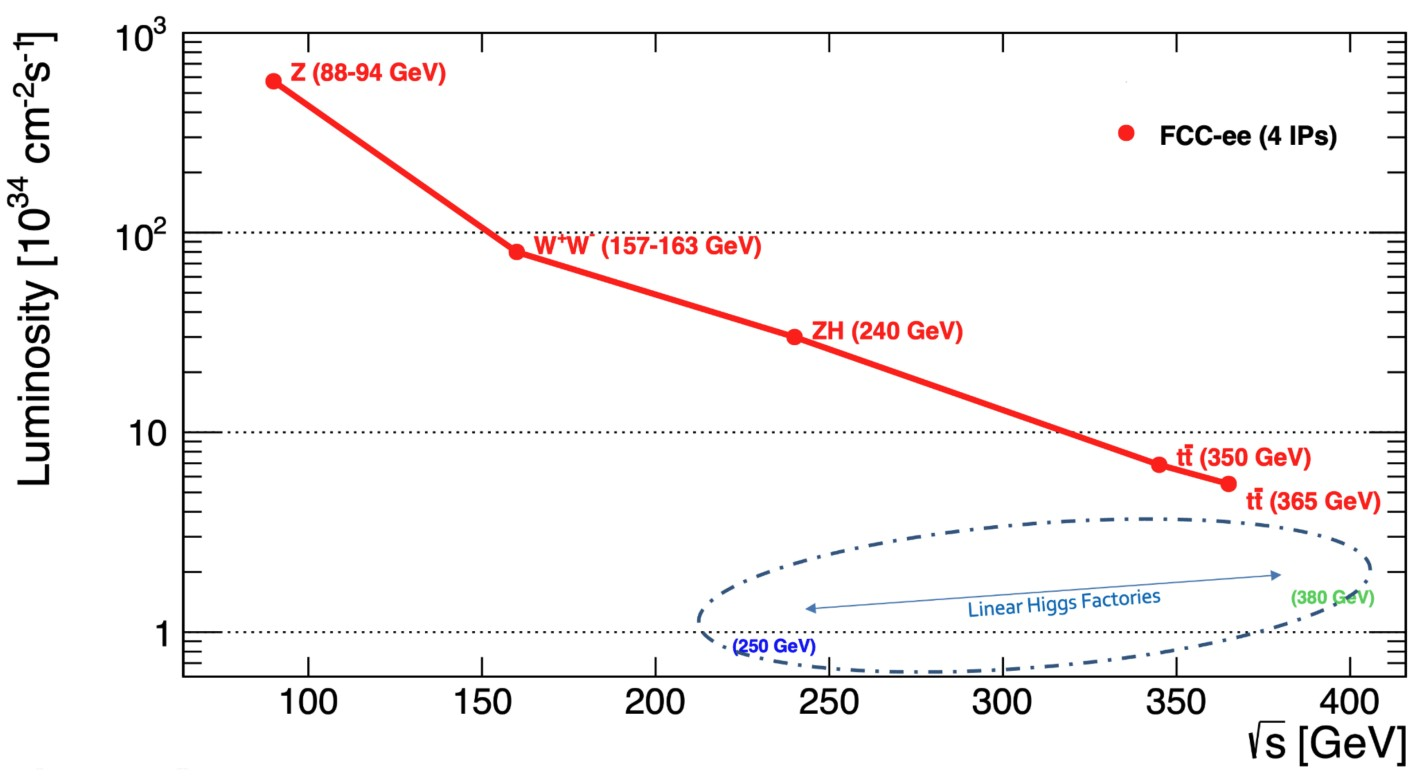
\includegraphics[width=\linewidth]{The_FCC_ee_baseline_design_luminosity}

%\vspace{0.25em}
			
{\scriptsize\justifying FCC-ee baseline design luminosity, summed over four interaction points, from the $Z$ pole to the $t\bar t$ threshold and beyond.\par}
\end{column}
		
\begin{column}{0.60\textwidth}
\scriptsize
\renewcommand{\arraystretch}{1.18}
\begin{tabularx}{\linewidth}{p{0.19\linewidth}p{0.22\linewidth}X}
\toprule
\textbf{Stage} & \textbf{$\sqrt{s}$} & \textbf{Main physics role}\\
\midrule
{\color{magenta}$Z$ pole} & 88, 91, 94~GeV & Tera-$Z$ programme: line shape, EW precision observables, heavy flavour, $\tau$ physics, QCD, rare $Z$ decays and dark-sector searches.\\
{\color{magenta}$WW$ threshold} & 157, 163~GeV & $m_W$, $\Gamma_W$, $W^+W^-$ threshold scan, diboson dynamics and inputs to EW/SMEFT fits.\\
{\color{magenta}$ZH$ Higgs stage} & 240~GeV & $e^+e^-\to ZH$ near the cross-section maximum: recoil method, $\kappa_Z$ anchor, absolute Higgs normalisation, invisible/exotic searches.\\
{\color{magenta}Top threshold and above} & 340-350, 365~GeV & $t\bar t$ threshold scan, $m_t$, $\Gamma_t$, $t\bar t Z$ couplings, $WW$-fusion input to Higgs fits, rare-top benchmarks.\\
\bottomrule
\end{tabularx}
\end{column}
\end{columns}
\vspace{0.35em}
\takehome{\justifying
The FCC-ee programme is not a single-energy Higgs factory: it is a sequence of precision laboratories for $Z$, $W$, Higgs and top physics, operated in the baseline scenario with four interaction points.}


\begin{tikzpicture}[remember picture,overlay]
\node[
anchor=north east,
xshift=-0.1cm,
yshift=-0.3cm
] at (current page.north east)
{
\includegraphics[width=1.8cm]{FCC.jpg}};
\end{tikzpicture}

\end{frame}







%----------------------------------------------------------------------------------------
\begin{frame}{FCC-ee baseline operation model: luminosity, and event yields}
\small
\begin{columns}[]%[T,totalwidth=\textwidth]
\begin{column}{0.50\textwidth}
\centering
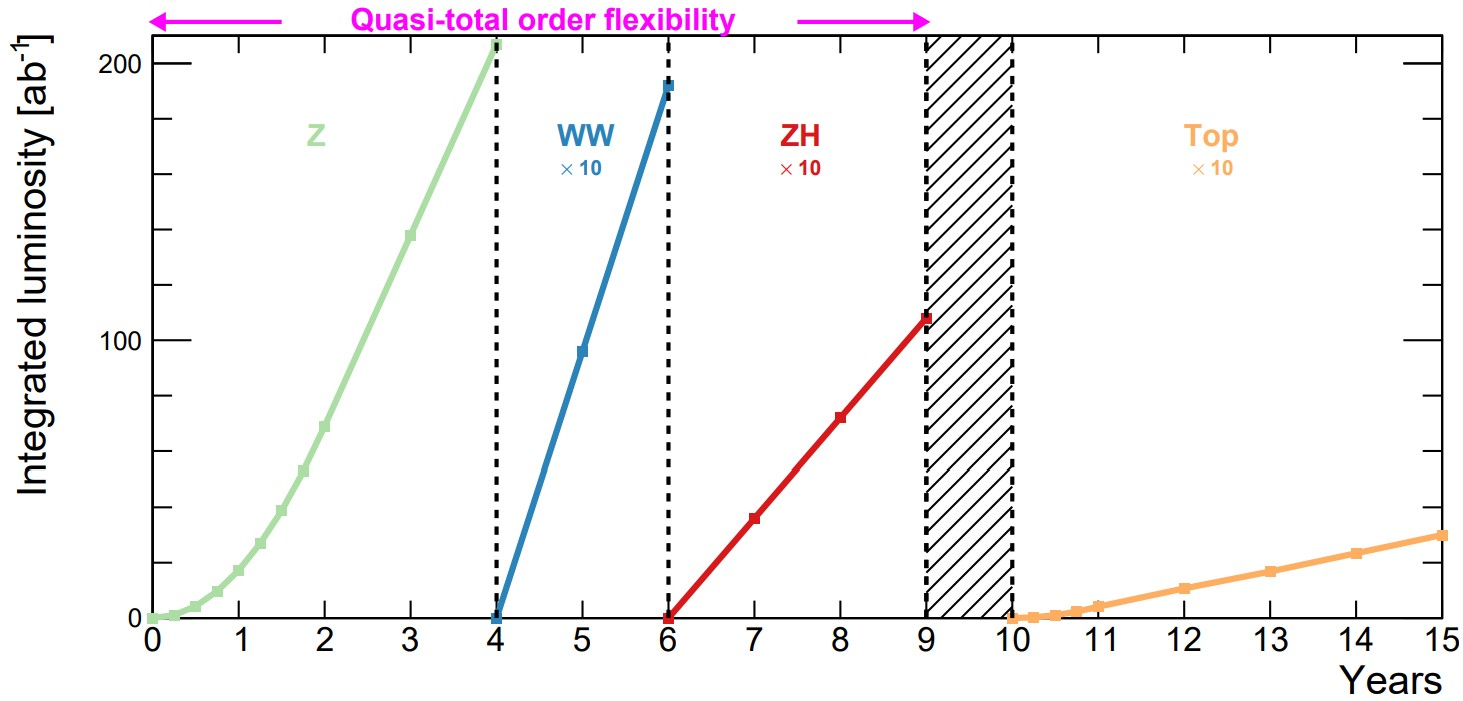
\includegraphics[width=\linewidth]{Baseline_operation_model_for_FCC_ee}
		
\scriptsize\justifying Example baseline luminosity evolution over about 15 years with four IPs. The shown order is illustrative; below the $t\bar t$ threshold the programme has quasi-total order flexibility.\par
\end{column}
		
\begin{column}{0.60\textwidth}
\scriptsize
\renewcommand{\arraystretch}{1.16}
\begin{tabularx}{\linewidth}{p{0.27\linewidth}p{0.23\linewidth}X}
\toprule
\textbf{Working point} & \textbf{Integrated lumi.} & \textbf{Baseline event sample}\\
\midrule
{\color{magenta}$Z$ pole} & $205~\mathrm{ab}^{-1}$ & $6\times10^{12}$ $Z$ bosons\\
{\color{magenta}$WW$ threshold} & $19.2~\mathrm{ab}^{-1}$ & $2.4\times10^8$ $WW$ events \\
{\color{magenta}$ZH$ stage} & $10.8~\mathrm{ab}^{-1}$ & $2.2\times10^6$ $ZH$ $+65\mathrm{k}$ $WW\to H$\\
{\color{magenta}$t\bar t$/365~GeV} & $0.42+2.70~\mathrm{ab}^{-1}$ & $2\times10^6$ $t\bar t$ $+370\mathrm{k}$ $ZH$ $+92\mathrm{k}$ $WW\to H$\\
\bottomrule
\end{tabularx}

\vspace{0.35em}

\begin{block}{Run-plan logic}
\scriptsize
\justifying
Four IPs give luminosity, detector diversity and redundancy against hidden systematics. Short early $Z/WW$ runs can commission the collider, detectors and resonant-depolarisation energy calibration; the high-statistics $Z$ programme remains the most demanding stage in accelerator, detector, theory and energy-control precision.
\end{block}
\end{column}
\end{columns}
\vspace{0.2em}
\takehome{\justifying
The baseline plan delivers a complete minimal FCC-ee physics programme within about 15 years, while keeping flexibility to optimise the order and duration of the $Z$, $WW$ and $ZH$ stages.}


\begin{tikzpicture}[remember picture,overlay]
\node[
anchor=north east,
xshift=-0.1cm,
yshift=-0.3cm
] at (current page.north east)
{
\includegraphics[width=1.8cm]{FCC.jpg}};
\end{tikzpicture}

\end{frame}




%----------------------------------------------------------------------------------------
\begin{frame}{FCC-ee precision mission: why the clean $e^+e^-$ stage matters}
\begin{columns}[T]%[T,totalwidth=\textwidth]
\begin{column}{0.50\textwidth}
\begin{block}{Machine-level advantages}
\begin{itemize}
\justifying 
\small 
\item clean \(e^+e^-\) initial state,
\item well-defined kinematics and beam-energy control,
%\item negligible pile-up and reduced QCD clutter,
\item full-event reconstruction with excellent flavor tagging potential.
\end{itemize}
\end{block}
			
\begin{block}{Physics mission}
\begin{itemize}
\justifying 
\small 
\item precision Z and W programme,
\item model-independent Higgs characterisation,
\item dedicated top-threshold and above-threshold measurements,
\item strong sensitivity to rare decays and forbidden interactions.
\end{itemize}
\end{block}
\end{column}
		
\begin{column}{0.55\textwidth}
\begin{tcolorbox}[colback=green!4,colframe=green!45!black,title=What makes FCC-ee special?]
\small
\justifying
FCC-ee combines \textbf{huge statistics}, \textbf{clean event reconstruction}, and 
\textbf{precise beam-energy control}.  With four interaction points, the programme gains 
luminosity, detector redundancy, and stronger control of hidden systematic biases.
\end{tcolorbox}
	
\begin{tcolorbox}[colback=white,colframe=black!30,title=Flagship precision goals]
\scriptsize
\justifying
\begin{itemize}\setlength\itemsep{0.25em}
\item \textbf{Tera-Z:} $6\times10^{12}$ $Z$ bosons for EW precision, flavour, QCD and rare-$Z$ searches.
\item \textbf{WW threshold:} sub-MeV access to $m_W$ and $\Gamma_W$, with gauge-sector constraints.
\item \textbf{ZH at 240~GeV:} recoil method and absolute normalisation of Higgs couplings through $\sigma(ZH)$.
\item \textbf{Top/365~GeV:} $m_t$, $\Gamma_t$, $t\bar t Z$ couplings and improved Higgs/EW global fits.
\end{itemize}
\end{tcolorbox}

\end{column}
\end{columns}


\begin{tikzpicture}[remember picture,overlay]
\node[
anchor=north east,
xshift=-0.1cm,
yshift=-0.3cm
] at (current page.north east)
{
\includegraphics[width=1.8cm]{FCC.jpg}};
\end{tikzpicture}

\end{frame}
%----------------------------------------------------------------------------------------






%\item For the FCNC study, the most relevant benchmarks are:
%\begin{itemize}
%	\justifying 
%	\item \(\sqrt{s}=240\,\mathrm{GeV}\): Higgs-factory stage,
%	\item \(\sqrt{s}=365\,\mathrm{GeV}\): top \& electroweak stage.
%\end{itemize}
%\justifying 
%\item Our top FCNC feasibility study uses the conservative internal benchmark \(5~\mathrm{ab}^{-1}\) at 240~GeV and \(1.5~\mathrm{ab}^{-1}\) at 365~GeV.






%----------------------------------------------------------------------------------------
\begin{frame}{The FCC integrated vision: precision first, discovery next}
\begin{center}
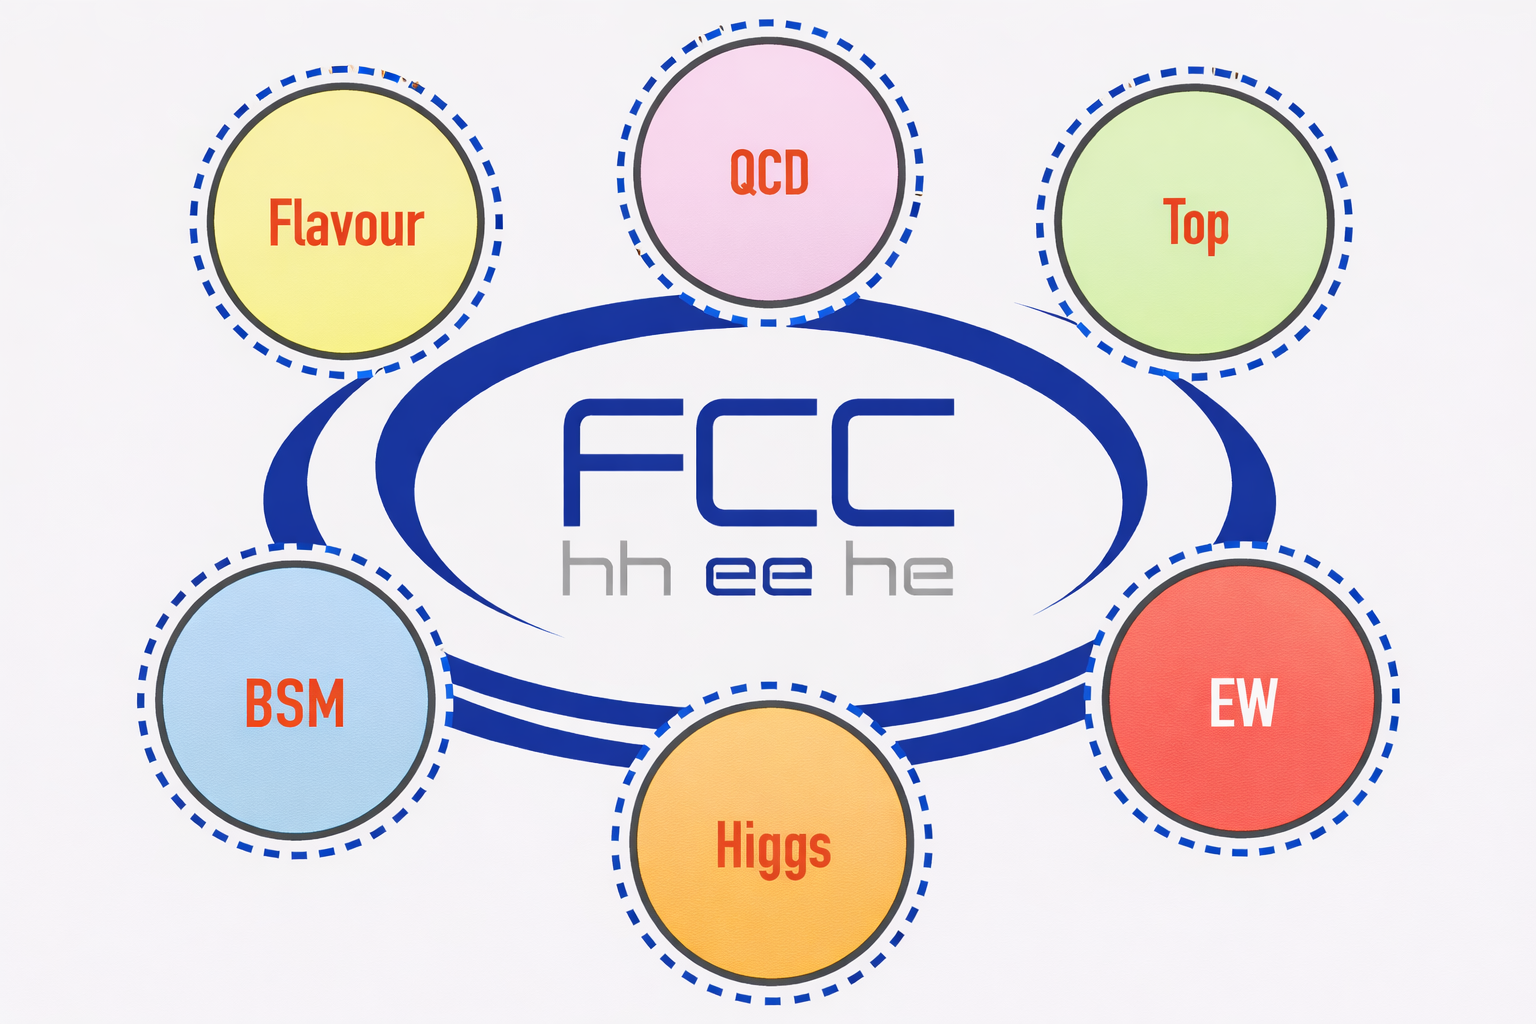
\includegraphics[width=0.70\linewidth]{FCC_ee_2.png}
\end{center}
\vspace{-0.4em}
\begin{itemize}
\item \justifying \small The integrated FCC programme lays out a long-term post-LHC strategy for exploring fundamental interactions: its first stage, FCC-ee, provides an exceptionally clean precision environment to test the Standard Model with unprecedented accuracy and to probe subtle signs of new physics.
\end{itemize}

\begin{tikzpicture}[remember picture,overlay]
\node[
anchor=north east,
xshift=-0.1cm,
yshift=-0.3cm
] at (current page.north east)
{
\includegraphics[width=1.8cm]{FCC.jpg}};
\end{tikzpicture}


\end{frame}
%----------------------------------------------------------------------------------------






%----------------------------------------------------------------------------------------
\begin{frame}{Why FCC-ee is a unique: Higgs factory, EW, top, BSM search}
\vspace{-0.4cm}
\begin{columns}[T]%[T,totalwidth=\textwidth]
	
\begin{column}{0.30\textwidth}
\begin{exampleblock}{Higgs}
\small
\justifying 
Model-independent \(ZH\) recoil measurements, absolute coupling extraction, width and invisible-decay sensitivity.
\end{exampleblock}
\end{column}

\begin{column}{0.30\textwidth}
\begin{block}{Electroweak}
\small
\justifying 
Ultra-high statistics at the Z pole and WW threshold enable precision tests of the gauge sector and flavour observables.
\end{block}
\end{column}

\begin{column}{0.30\textwidth}
\begin{alertblock}{Top}
\small
\justifying 
Threshold and above-threshold running provide precision access to the top mass, width, electroweak couplings and rare-top observables.
\end{alertblock}
\end{column}

\end{columns}

\vspace{-0.1cm}

\begin{tcolorbox}[colback=white,colframe=blue!50!black,boxrule=0.8pt,arc=2mm]
\small
\justifying
FCC-ee BSM programme: The same clean \(e^+e^-\) environment and precision strategy make FCC-ee a powerful machine for indirect and rare-process searches beyond the Standard Model, including EFT deviations, precision electroweak anomalies, and forbidden top interactions.
\end{tcolorbox}

\vspace{-0.3cm}

\begin{tcolorbox}[colback=white,colframe=red!30]
\small
\justifying 
The key FCC-ee idea is \textbf{precision with interpretation}: huge $Z$, $W$, Higgs and top samples 
are combined with clean kinematics, beam-energy control and full-event reconstruction to extract 
absolute couplings, widths and electroweak vertices, and to test correlated SMEFT deviations.
\end{tcolorbox}

\end{frame}







%----------------------------------------------------------------------------------------
\begin{frame}{Tera-$Z$: the electroweak precision anchor}
	
\begin{columns}[T]%[T,totalwidth=\textwidth]
	
\begin{column}{0.60\textwidth}
\begin{itemize}
\justifying
\small
\item The $Z$ line-shape scan and $6\times10^{12}$ $Z$ bosons provide an EW precision programme far beyond LEP/SLC.
\item Central observables include $m_Z$, $\Gamma_Z$, $\sin^2\theta_{\rm eff}^W$, $R_\ell^Z$, $\sigma^0_{\rm had}$, $N_\nu$, $R_b$, heavy-flavour asymmetries and $\tau$ observables.
\item Off-peak running around the $Z$ pole also gives direct handles on $\alpha_{\rm QED}(m_Z)$ and $\alpha_s(m_Z)$.
\end{itemize}
\end{column}


\begin{column}{0.50\textwidth}
\centering
\scriptsize
\begin{tabular}{lcc}
\toprule
Observable & FCC-ee stat. & FCC-ee syst. \\
\midrule
$m_Z$ & $4~\mathrm{keV}$ & $100~\mathrm{keV}$ \\
$\Gamma_Z$ & $4~\mathrm{keV}$ & $12~\mathrm{keV}$ \\
$\sin^2\theta_{\rm eff}^W$ & $1.2\times10^{-6}$ & $1.2\times10^{-6}$ \\
$N_\nu$ & $0.09\times10^{-3}$ & $0.12\times10^{-3}$ \\
$R_b$ & $0.25\times10^{-6}$ & $0.3\times10^{-6}$ \\
\bottomrule
\end{tabular}
\vspace{0.25cm}

\begin{block}{Message}
\small
The $Z$ pole is both a discovery programme and the EW calibration layer for Higgs physics.
\end{block}
\end{column}


\end{columns}


\end{frame}



%----------------------------------------------------------------------------------------
\begin{frame}{From $Z$ observables to electroweak couplings}
\begin{columns}[T,totalwidth=\textwidth]
\begin{column}{0.55\textwidth}
\begin{itemize}
\justifying
\small
\item FCC-ee determines left- and right-handed $Zf\bar f$ couplings from partial widths, cross-section ratios and asymmetries.
\item For electrons, this is especially important because the $Zee$ vertex also enters $e^+e^-\to ZH$.
\item In SMEFT, new-physics effects in $Zee$ and $HZee$ are correlated by electroweak gauge invariance.
\end{itemize}
\vspace{0.2cm}
\begin{block}{Extraction logic}
\centering
$g_{Zf}^{L,R}\ \longleftarrow\ \Gamma(Z\to f\bar f),\ A_f,\ A_{\rm FB}^f,\ R_f,\ P_\tau$
\end{block}
\end{column}
\begin{column}{0.42\textwidth}
\begin{block}{Why chirality matters}
\small
\begin{itemize}
\justifying
\item $g_L$ and $g_R$ enter different combinations in rates and asymmetries;
\item BSM effects often appear as chiral shifts;
\item Higgs fits need EW vertices known at comparable precision.
\end{itemize}
\end{block}
\begin{alertblock}{Practical consequence}
\small
Without FCC-ee $Z$-pole precision, uncertainties in EW vertices would contaminate the extraction of Higgs couplings.
\end{alertblock}
\end{column}
\end{columns}
\refs{FCC Feasibility Study Report Vol.~1, Sec.~2.2.1.}
\end{frame}



%----------------------------------------------------------------------------------------
\begin{frame}{WW threshold: precision W physics and gauge structure}
\begin{columns}[T,totalwidth=\textwidth]
\begin{column}{0.52\textwidth}
\begin{itemize}
\justifying
\small
\item A scan near the $W^+W^-$ threshold gives a sub-MeV determination of $m_W$ and $\Gamma_W$.
\item Above threshold, $e^+e^-\to W^+W^-$ probes the gauge-boson self-interactions and diboson angular structure.
\item In SMEFT, anomalous triple-gauge couplings such as $\delta g_{1,Z}$ and $\delta\kappa_\gamma$ are correlated with $HVV$ interactions.
\end{itemize}
\end{column}
\begin{column}{0.45\textwidth}
\centering
\scriptsize
\begin{tabular}{lcc}
\toprule
Observable & FCC-ee stat. & FCC-ee syst. \\
\midrule
$m_W$ & $0.18~\mathrm{MeV}$ & $0.16~\mathrm{MeV}$ \\
$\Gamma_W$ & $0.27~\mathrm{MeV}$ & $0.20~\mathrm{MeV}$ \\
$\alpha_s(m_W^2)$ & $2\times10^{-4}$ & $2\times10^{-4}$ \\
$N_\nu$ & $0.5\times10^{-3}$ & small \\
\bottomrule
\end{tabular}
\vspace{0.25cm}
\begin{block}{Message}
\small
The $WW$ programme constrains the gauge structure that also controls Higgs-sector interpretation.
\end{block}
\end{column}
\end{columns}
\refs{FCC Feasibility Study Report Vol.~1, Table~2 and Sec.~2.2.2.}
\end{frame}



%----------------------------------------------------------------------------------------
\begin{frame}{Why $Z$ and $WW$ precision sharpen Higgs coupling extraction}

\vspace{-0.4cm}

\begin{columns}[T]%[T,totalwidth=\textwidth]
	
\begin{column}{0.55\textwidth}
\centering
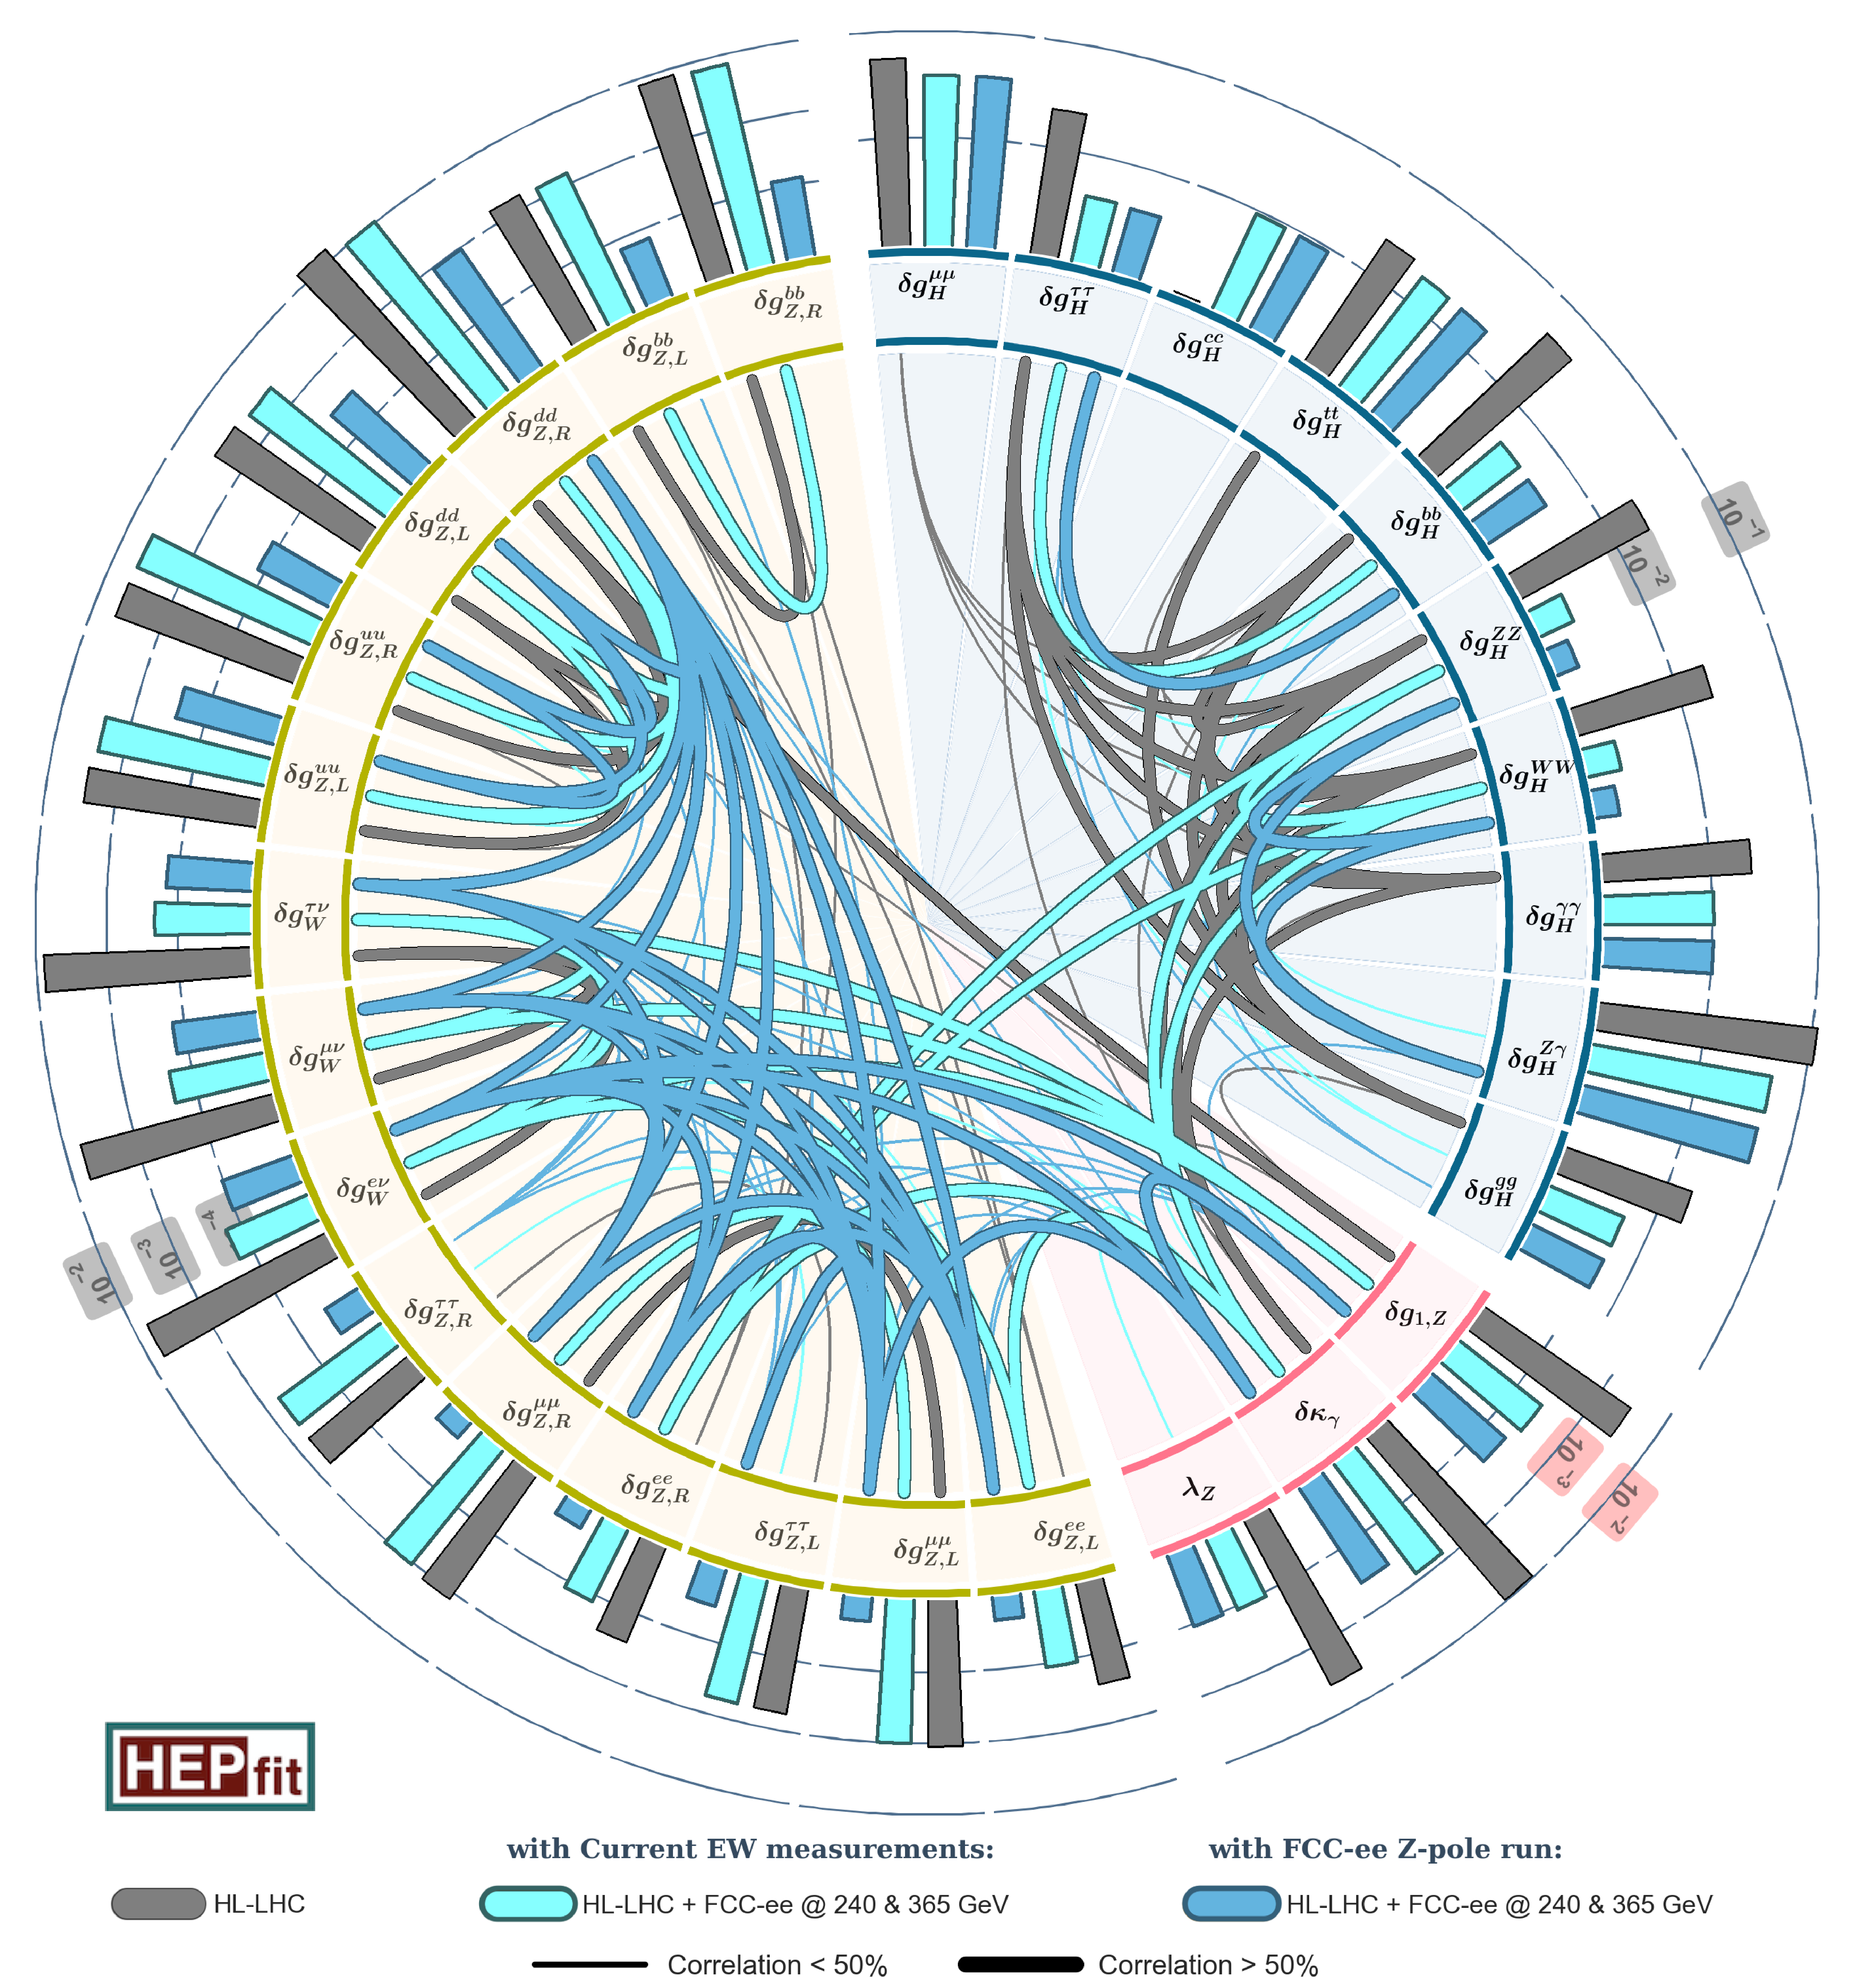
\includegraphics[width=1.1\linewidth]{circos_FCCee_nomargin_newFSR.pdf}
\end{column}

\begin{column}{0.50\textwidth}
\begin{itemize}
\justifying
\small
\item The same SMEFT operators can affect EW vertices, aTGCs and Higgs production.
\item $Z$-pole data reduce correlations between the Higgs and EW sectors.
\item With only LEP/SLC-level EW information, some 240~GeV Higgs-coupling precisions would deteriorate by up to about a factor of two.
\item Diboson data constrain aTGC directions correlated with $HZZ$ and $HWW$.
\end{itemize}

\begin{alertblock}{Message}
\small
The $Z$ and $WW$ runs are not pre-Higgs extras; they are part of the Higgs measurement.
\end{alertblock}

\end{column}
\end{columns}
%\refs{FCC Feasibility Study Report Vol.~1, Fig.~4 and Secs.~2.2.1--2.2.2.}
\end{frame}





%----------------------------------------------------------------------------------------
\begin{frame}{The $ZH$ stage at 240 GeV: the Higgs standard candle}
\begin{columns}[T,totalwidth=\textwidth]
\begin{column}{0.52\textwidth}
\begin{itemize}
\justifying
\small
\item At $\sqrt{s}\simeq240~\mathrm{GeV}$, $e^+e^-\to ZH$ is near its cross-section maximum.
\item Reconstructing the $Z$ gives the Higgs recoil mass independently of the Higgs decay mode:
\[
m_{\rm recoil}^2=s+m_Z^2-2\sqrt{s}\,E_Z .
\]
\item The inclusive $\sigma(ZH)$ measurement anchors $\kappa_Z$ and the absolute normalisation of Higgs couplings.
\item The recoil method also enables invisible and exotic Higgs-decay searches.
\end{itemize}
\end{column}
\begin{column}{0.45\textwidth}
\centering
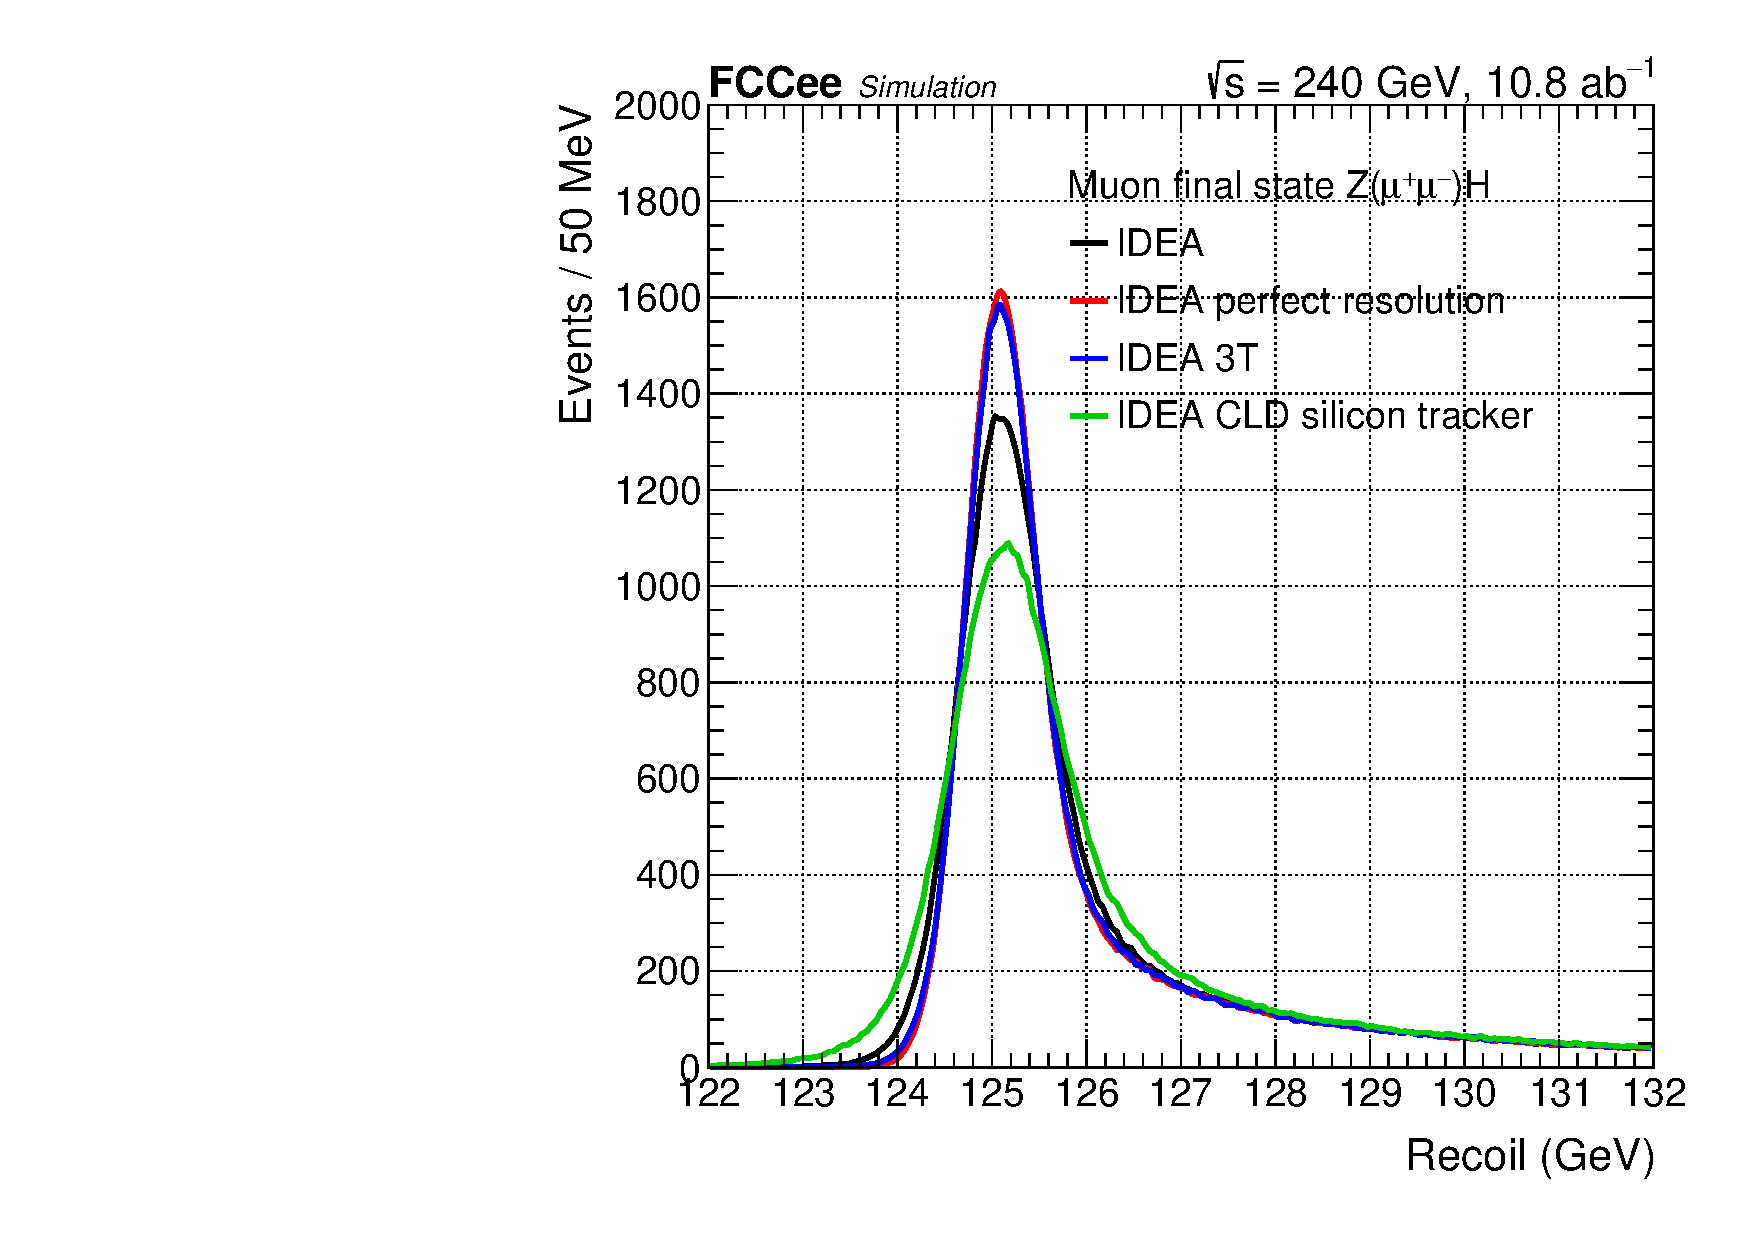
\includegraphics[width=0.93\linewidth]{HiggsRecoil_IDEA_IDEAL_2T_3T_CLD_mumu_mrec.pdf}
\vspace{0.1cm}
\begin{block}{Foundation}
\centering\small
$\sigma(ZH)$ is measured inclusively: no assumption on the Higgs decay is required.
\end{block}
\end{column}
\end{columns}
\refs{FCC Feasibility Study Report Vol.~1, Secs.~1.1, 2.2 and Detector Requirements.}
\end{frame}



%----------------------------------------------------------------------------------------
\begin{frame}{Higgs coupling and width extraction: the logic}
\begin{columns}[T,totalwidth=\textwidth]
\begin{column}{0.53\textwidth}
\begin{block}{Measured rates}
\small
				\[
				\sigma(ZH),\qquad \sigma(ZH)\times {\rm BR}(H\to X),
				\]
				\[
				\sigma(\nu\bar\nu H)\times {\rm BR}(H\to X) \quad (\text{higher }\sqrt{s}).
				\]
\end{block}
\begin{block}{Coupling scaling}
\small
				\[
				\sigma(ZH)\propto \kappa_Z^2,
				\qquad
				\sigma(ZH){\rm BR}(H\to b\bar b)
				\propto \frac{\kappa_Z^2\kappa_b^2}{\Gamma_H}.
				\]
\end{block}
\end{column}
\begin{column}{0.44\textwidth}
\begin{itemize}
\justifying
\small
\item Inclusive $ZH$ fixes the absolute production normalisation.
\item Exclusive decays map partial widths: $b\bar b$, $c\bar c$, $gg$, $\tau\tau$, $WW^*$, $ZZ^*$, $\gamma\gamma$, $Z\gamma$, $\mu\mu$.
\item Combining $ZH$ and vector-boson-fusion information gives model-independent access to $\Gamma_H$.
\item Invisible and untagged modes are constrained by recoil and global fits.
\end{itemize}
\end{column}
\end{columns}
\takehome{FCC-ee turns Higgs rates into absolute couplings because $\sigma(ZH)$ is measured inclusively.}
\refs{FCC Feasibility Study Report Vol.~1, Sec.~1.1 and Table~3.}
\end{frame}




%----------------------------------------------------------------------------------------
\begin{frame}{Projected Higgs precision and HL-LHC comparison}
\begin{columns}[T,totalwidth=\textwidth]
\begin{column}{0.52\textwidth}
\centering
\scriptsize
\begin{tabular}{lccc}
\toprule
Quantity & HL-LHC & FCC-ee & FCC-ee+FCC-hh \\
\midrule
$\kappa_Z$ & $1.3\%^{*}$ & $0.10\%$ & $0.10\%$ \\
$\kappa_W$ & $1.5\%^{*}$ & $0.29\%$ & $0.25\%$ \\
$\kappa_b$ & $2.5\%^{*}$ & $0.38/0.49\%$ & $0.33/0.45\%$ \\
$\kappa_c$ & -- & $0.70/0.87\%$ & $0.68/0.85\%$ \\
$\kappa_\tau$ & $1.6\%^{*}$ & $0.46\%$ & $0.40\%$ \\
$\Gamma_H$ & -- & $0.78\%$ & $0.69\%$ \\
$B_{\rm inv}$ 95\% CL & $1.9\times10^{-2*}$ & $5\times10^{-4}$ & $2.3\times10^{-4}$ \\
\bottomrule
\end{tabular}
\vspace{0.1cm}
\scriptsize $^{*}$HL-LHC coupling interpretation uses assumptions such as $|\kappa_V|\leq1$.
\end{column}
\begin{column}{0.45\textwidth}
\begin{itemize}
\justifying
\small
\item FCC-ee provides absolute coupling normalisation through inclusive $ZH$.
\item Key vector couplings enter the per-mille regime.
\item FCC-hh later adds rare modes, top Yukawa and double-Higgs sensitivity.
\item The programme is complementary to HL-LHC, not a replacement for it.
\end{itemize}
\begin{alertblock}{Message}
\small
FCC-ee moves central Higgs observables from percent-level to sub-percent or per-mille precision.
\end{alertblock}
\end{column}
\end{columns}
\refs{FCC Feasibility Study Report Vol.~1, Table~3.}
\end{frame}








%----------------------------------------------------------------------------------------
\begin{frame}{Why the 365 GeV/top stage matters for Higgs precision}
\begin{columns}[T,totalwidth=\textwidth]
\begin{column}{0.52\textwidth}
\begin{itemize}
\justifying
\small
\item Higher-energy running increases the importance of $WW$ fusion, improving $\kappa_W$ and $\Gamma_H$ constraints.
\item The $ZH$ cross-section dependence on $\sqrt{s}$ provides indirect sensitivity to the Higgs self-coupling in global fits.
\item A $t\bar t$ threshold scan gives precise $m_t$ and $\Gamma_t$, reducing parametric limitations in EW predictions.
\item Above threshold, $t\bar t Z$ couplings can be measured at the $0.5$--$1.5\%$ level.
\end{itemize}
\end{column}
\begin{column}{0.45\textwidth}
\centering
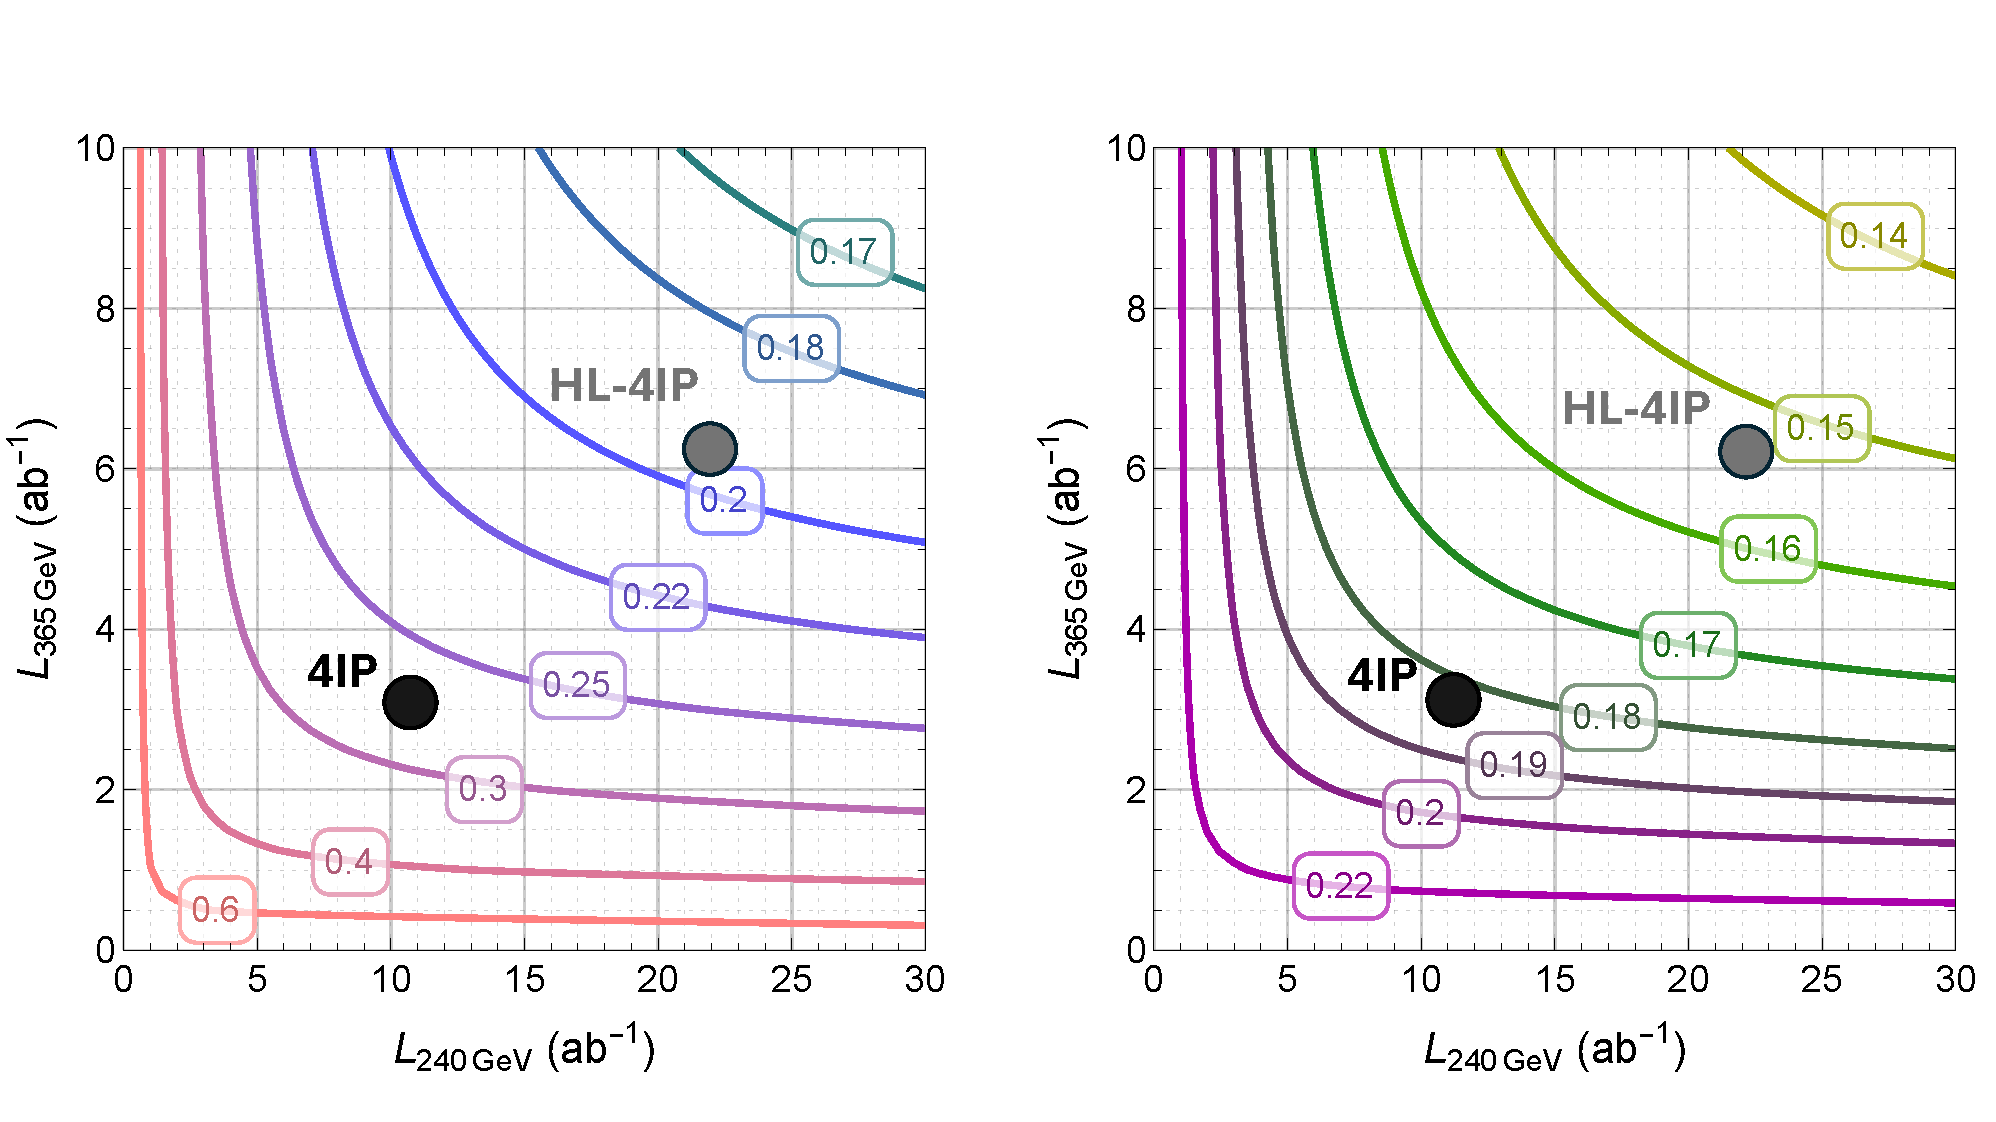
\includegraphics[width=0.88\linewidth]{Hselfcoupling-precision-1b.pdf}
\vspace{0.1cm}
\begin{block}{Message}
\small
The 365~GeV stage is not only a top run; it sharpens the global Higgs/EW interpretation.
\end{block}
\end{column}
\end{columns}
\refs{FCC Feasibility Study Report Vol.~1, Table~2 and Secs.~2.2.3--2.2.4.}
\end{frame}










%----------------------------------------------------------------------------------------
\begin{frame}{SMEFT view: precision as a high-scale microscope}
\begin{columns}[T,totalwidth=\textwidth]
\begin{column}{0.56\textwidth}
\centering
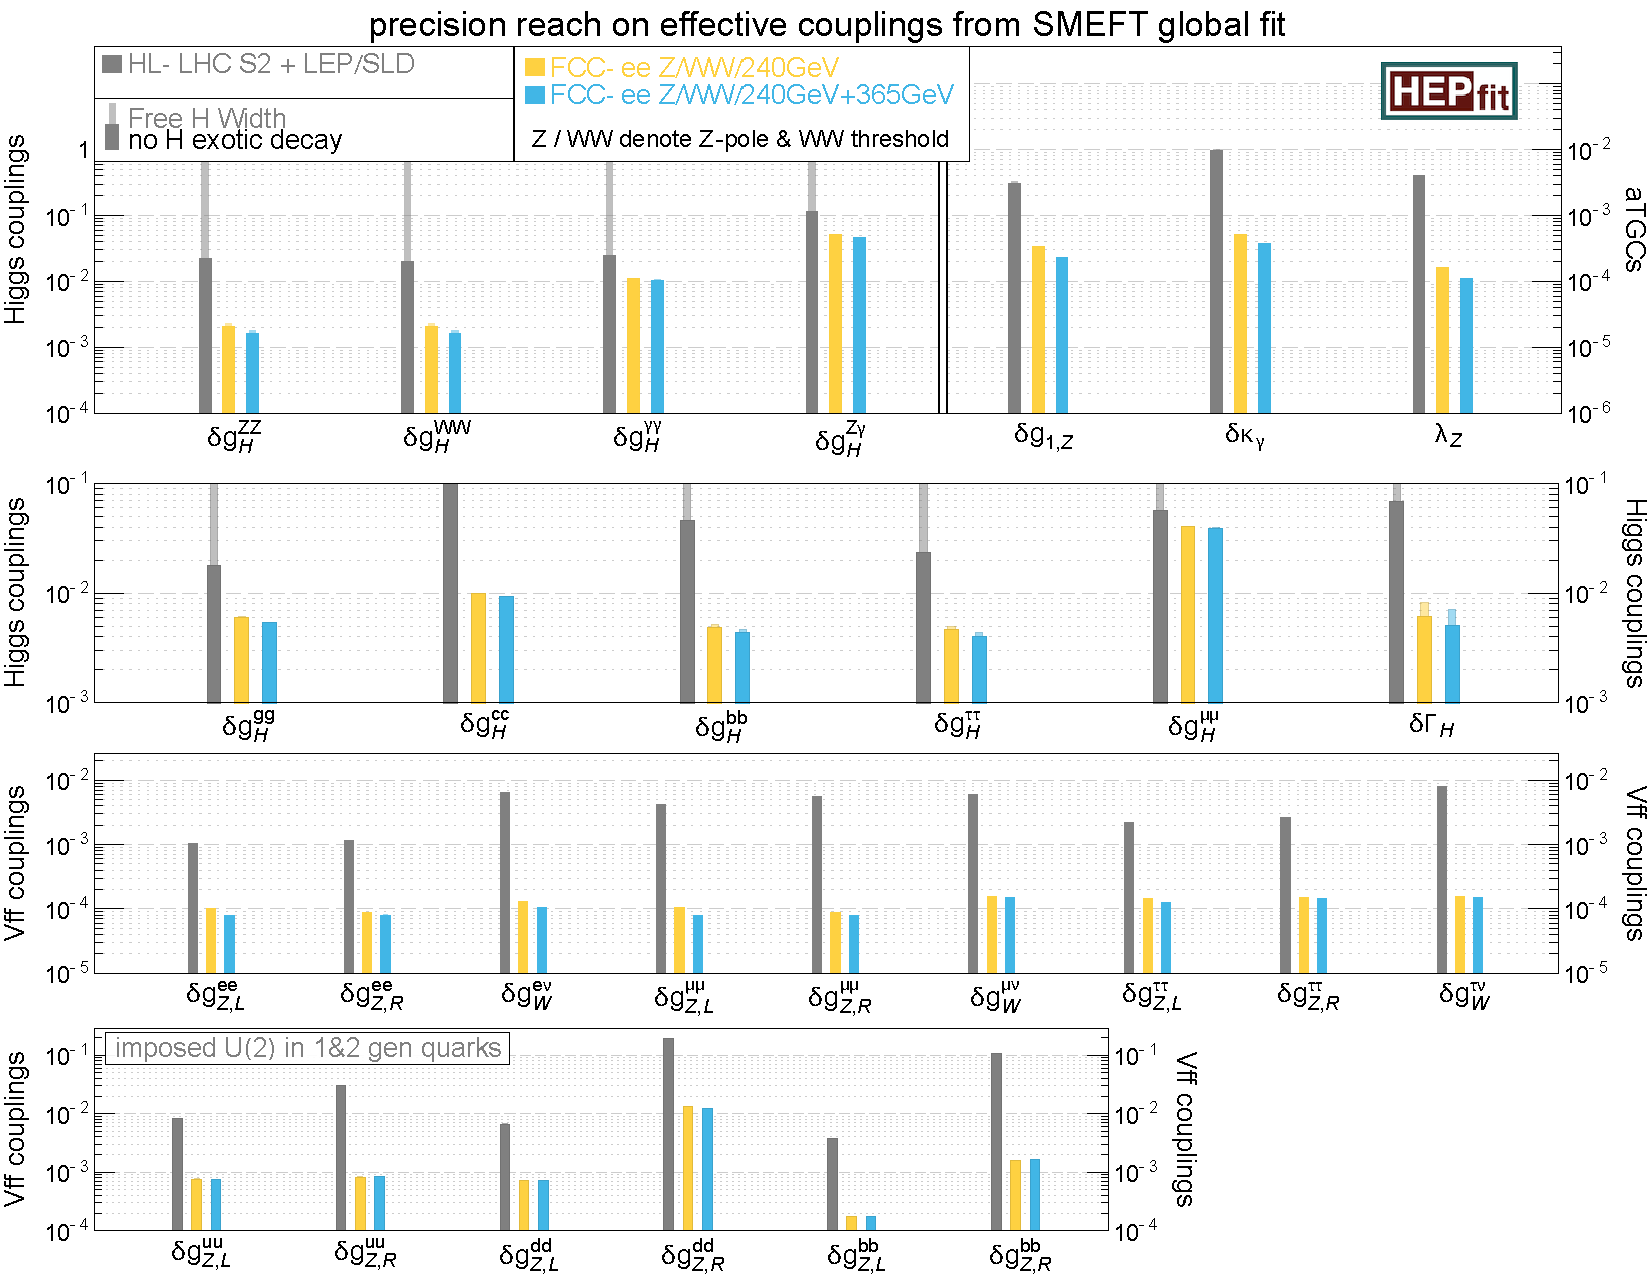
\includegraphics[width=0.98\linewidth]{barplotsnow-xo1-smpar_newFSR-CL.pdf}
\end{column}
\begin{column}{0.40\textwidth}
\begin{itemize}
\justifying
\small
\item SMEFT parameterises heavy new physics through dimension-6 operators and Wilson coefficients.
\item Gauge invariance correlates deviations across $Zf\bar f$, $WW$, $ZH$, $\nu\bar\nu H$ and $t\bar t$ observables.
\item FCC-ee precision tests \alert{patterns of deviations}, not only individual signal strengths.
\item A null result still strongly constrains broad classes of BSM scenarios.
\end{itemize}
\begin{block}{Fit ingredients}
\small EWPOs + light-fermion pairs + Higgs + diboson + top data.
\end{block}
\end{column}
\end{columns}
\refs{FCC Feasibility Study Report Vol.~1, Fig.~3 and Sec.~2.2.}
\end{frame}




%----------------------------------------------------------------------------------------
\begin{frame}{The top programme at FCC-ee: threshold, electroweak couplings, and Yukawa sensitivity}
\begin{columns}[T,totalwidth=\textwidth]
\begin{column}{0.50\textwidth}
\begin{itemize}
\justifying 
\small
\item The top-threshold scan is designed for precision extraction of \(m_t\), \(\Gamma_t\), and strong-interaction inputs.
\item Above threshold, the 365~GeV stage enhances sensitivity to \alert{top electroweak couplings} and to the \alert{top Yukawa} through indirect and kinematic handles.
\item Together, threshold and above-threshold measurements create a coherent top programme rather than a single ``top point''.
\item Rare-top probes such as FCNC complement these precision observables by testing interactions that are essentially absent in the SM.
\end{itemize}
\end{column}
\begin{column}{0.46\textwidth}
\begin{table}
\centering
\scriptsize
\renewcommand{\arraystretch}{1.2}
\resizebox{0.95\linewidth}{!}{%
\begin{tabular}{lcccc}
\hline\hline
\textbf{Observable} & \multicolumn{2}{c}{\textbf{Present}} & \textbf{FCC-ee} & \textbf{FCC-ee} \\
& \textbf{value} & \textbf{uncertainty} & \textbf{Stat.} & \textbf{Syst.} \\
\hline
$m_{\mathrm{top}}$ (MeV)      & 172570 & $\pm\,290$        & \textbf{4.2}        & 4.9 \\
$\Gamma_{\mathrm{top}}$ (MeV) & 1420   & $\pm\,190$        & \textbf{10.0}       & 6.0 \\
$y_{\mathrm{top}}$            & --     & $\pm\,10\%$       & \textbf{1.5\%}      & 1.5\% \\
$g_{ttZ}$ (L-R)               & --     & $\pm\,10$--$30\%$ & \textbf{0.5$-$1.5\%} & small \\
\hline\hline
\end{tabular}%
}
\end{table}
\vspace{-0.2cm}
\begin{block}{Message from top-threshold}
\small
\justifying
FCC-ee top-threshold and above-threshold running together define a genuine precision top programme. 
The projected sensitivities show dramatic improvements in the determination of \(m_t\), \(\Gamma_t\), 
\(y_t\), and \(g_{ttZ}\), making FCC-ee a powerful machine for both Standard Model tests and indirect new-physics searches.
\end{block}
\end{column}
\end{columns}
\refs{\textit{M. M. Defranchis et al., {\color{magenta}A detailed study on the prospects for a \(t\bar t\) threshold scan in \(e^+e^-\) collisions}, JHEP 11 (2025) 020}; \textit{M. Selvaggi, A. Blondel, J. Eysermans, {\color{magenta}Prospects in Electroweak, Higgs and Top physics at FCC}}.}
\end{frame}






%----------------------------------------------------------------------------------------
\begin{frame}{Why top and Higgs precision sharpen indirect BSM sensitivity}
\begin{columns}[T,totalwidth=\textwidth]
\begin{column}{0.50\textwidth}
\begin{block}{Precision side}
\small 
\justifying 
Higgs and top precision measurements can reveal small departures from the Standard Model and therefore provide an indirect window on new physics. 
\end{block}
\begin{alertblock}{Rare-process side}
\small 
\justifying 
FCNC transitions in the top sector are essentially absent at tree level in the Standard Model; any signal would be a direct pointer to BSM dynamics.
\end{alertblock}
\end{column}
\begin{column}{0.46\textwidth}
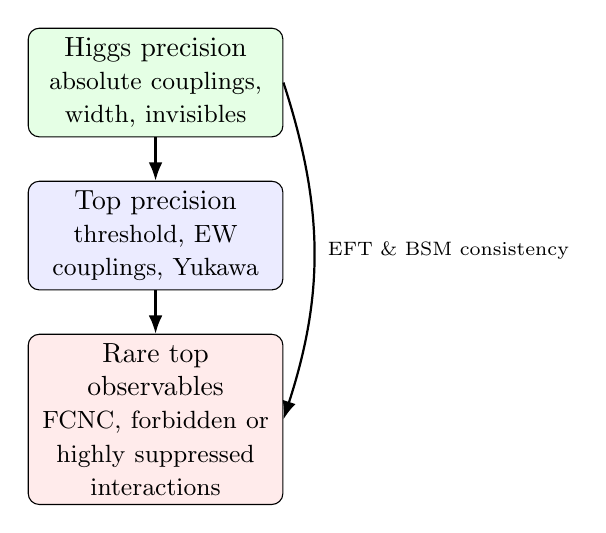
\begin{tikzpicture}[node distance=1.25cm,>=Latex, every node/.style={align=center},node distance=0.55cm]
\node[draw,rounded corners,fill=green!10,text width=3.0cm,minimum height=0.9cm] (h) {Higgs precision\\\small absolute couplings, width, invisibles};
\node[draw,rounded corners,fill=blue!8,text width=3.0cm,minimum height=0.9cm,below=of h] (t) {Top precision\\\small threshold, EW couplings, Yukawa};
\node[draw,rounded corners,fill=red!8,text width=3.0cm,minimum height=0.9cm,below=of t] (f) {Rare top observables\\\small FCNC, forbidden or highly suppressed interactions};
\draw[->,thick] (h) -- (t);
\draw[->,thick] (t) -- (f);
\draw[->,thick,bend left=18] (h.east) to node[right,font=\scriptsize]{\,EFT \& BSM consistency} (f.east);
\end{tikzpicture}
\end{column}
\end{columns}
%\takehome{
%\justifying 
%In this logic, top FCNC is not an add-on to the FCC-ee physics case --- it is one of its cleanest BSM stress tests.}
%\refs{FCC integrated-programme logic; top-FCNC EFT literature.}
\end{frame}






%----------------------------------------------------------------------------------------
\section{{\color{white}top-quark FCNC motivation and theory}}


\begin{frame}{FCNC in the Standard Model and beyond}
\begin{columns}[T,totalwidth=\textwidth]
\begin{column}{0.54\textwidth}
\begin{itemize}
\justifying 
\item In the SM, top FCNC interactions are \alert{absent at tree level} and strongly suppressed at one loop by the GIM mechanism.
\item Expected branching ratios are extraordinarily small - many channels lie around \(10^{-12}\)or smaller, which places them far beyond the reach of current experiments and even most future collider programmes. 
\item A measurable rate for \(t\to qV\) with \(X=\gamma,Z,H,g\) would therefore be a clear sign of physics beyond the Standard Model.
\item Many BSM scenarios can enhance the top-FCNC rates to experimentally interesting levels.
\end{itemize}
\end{column}
\begin{column}{0.43\textwidth}
\centering
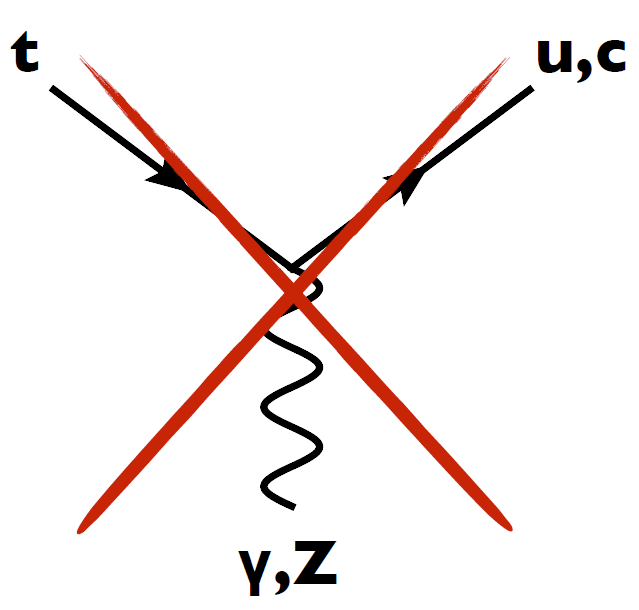
\includegraphics[width=0.31\linewidth]{Presentation_Higgs_performance_meeting19marc_2024/FCNC_SM.png}\hfill
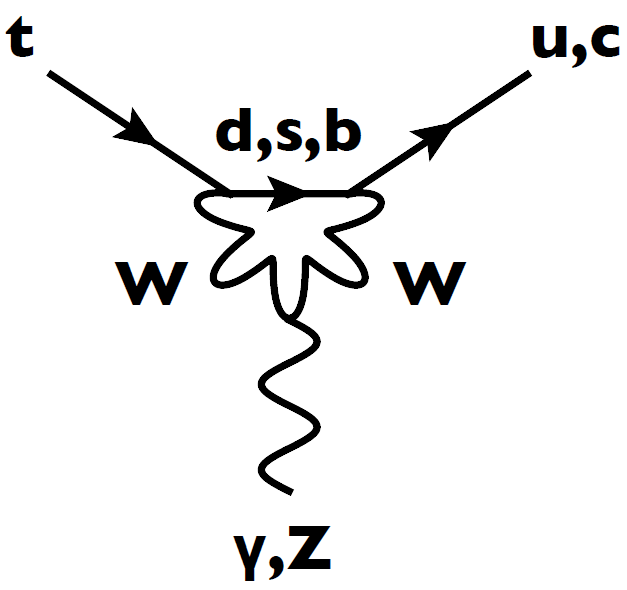
\includegraphics[width=0.31\linewidth]{Presentation_Higgs_performance_meeting19marc_2024/FCNC_SM_loop.png}\hfill
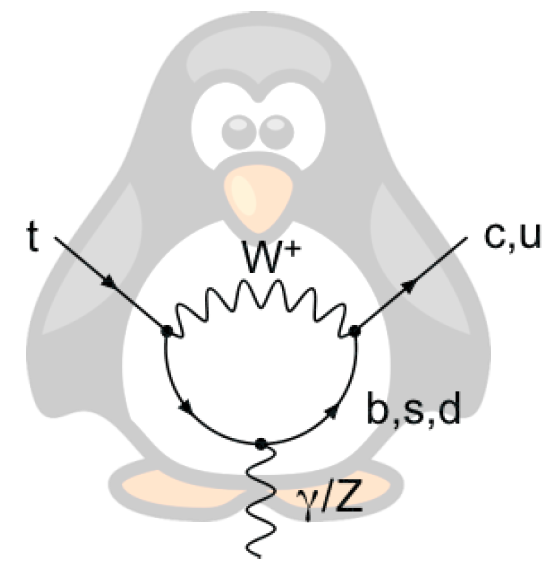
\includegraphics[width=0.31\linewidth]{Presentation_Higgs_performance_meeting19marc_2024/FCNC_SM_pin.png}
\vspace{0.5em}
\begin{tcolorbox}[colback=white,colframe=black!30]
\small
SM: tiny rates\\
BSM: potentially enhanced rates\\
\centering
\textbf{Any signal \(\Rightarrow\) new physics.}
\end{tcolorbox}
\end{column}
\end{columns}
\vspace{0.2cm}
\refs{Aguilar-Saavedra, Acta Phys. Polon. B35 (2004) 2695; internal analysis note.}
\end{frame}






%----------------------------------------------------------------------------------------
\begin{frame}{Why top FCNC is a powerful BSM probe}
\begin{columns}[T,totalwidth=\textwidth]
\begin{column}{0.57\textwidth}
\begin{itemize}
\justifying 
\item The top quark is the heaviest SM fermion and has a particularly intimate connection to electroweak symmetry breaking.
\item New heavy dynamics can leave visible traces in the top sector even when no new state is produced on shell.
\item FCNC processes probe flavor, chirality and gauge structure simultaneously.
\item At FCC-ee the signal process is especially clean because the initial state is known and the dominant hadronic clutter of hadron colliders is absent.
\end{itemize}
\end{column}
\begin{column}{0.40\textwidth}
\centering
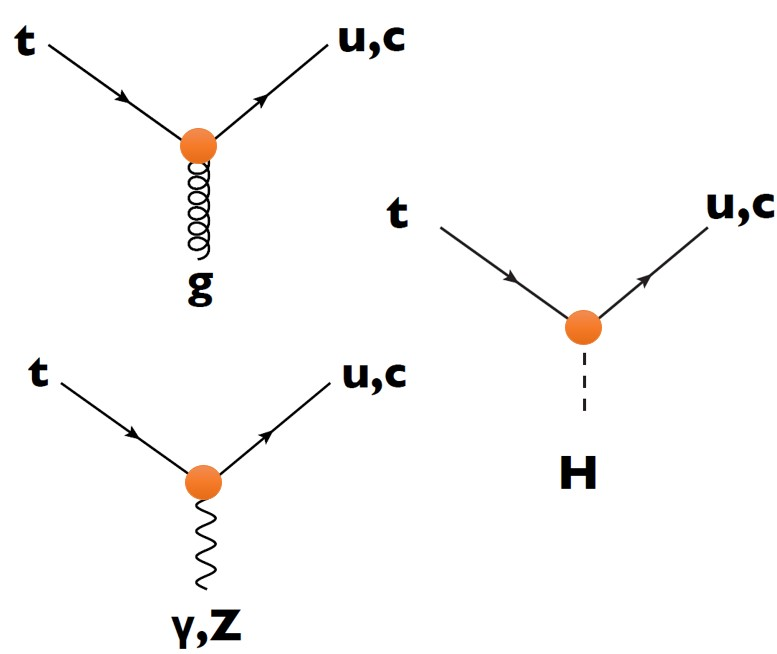
\includegraphics[width=\linewidth]{FCNC}
\end{column}
\end{columns}
%\refs{Top-FCNC anomalous-coupling literature; internal presentation assets.}
\begin{block}{Practical implication}
\small 
\justifying 
A single-top FCNC search at FCC-ee can turn small anomalous \(tq\gamma\) and \(tqZ\) couplings into visible rate distortions with controllable backgrounds.
\end{block}
\end{frame}






%----------------------------------------------------------------------------------------
\begin{frame}{Experimental status: LEP, LHC, and future prospects}
\begin{columns}[T,totalwidth=\textwidth]
\begin{column}{0.50\textwidth}
\begin{itemize}
\justifying 
\item LEP set the first direct limits on rare top interactions, but was far from the SM expectation.
\item ATLAS and CMS have pushed several top-FCNC bounds into the \(10^{-5}\)-\(10^{-4}\) range, depending on the channel.
\item The strongest present limits are already testing interesting BSM territory, especially in \(t\to q\gamma\), \(t\to qZ\), and \(t\to qH\).
\item FCC-ee probes the same physics with a completely different experimental environment and therefore a different systematics / background profile.
\end{itemize}
\end{column}
\begin{column}{0.47\textwidth}
\centering
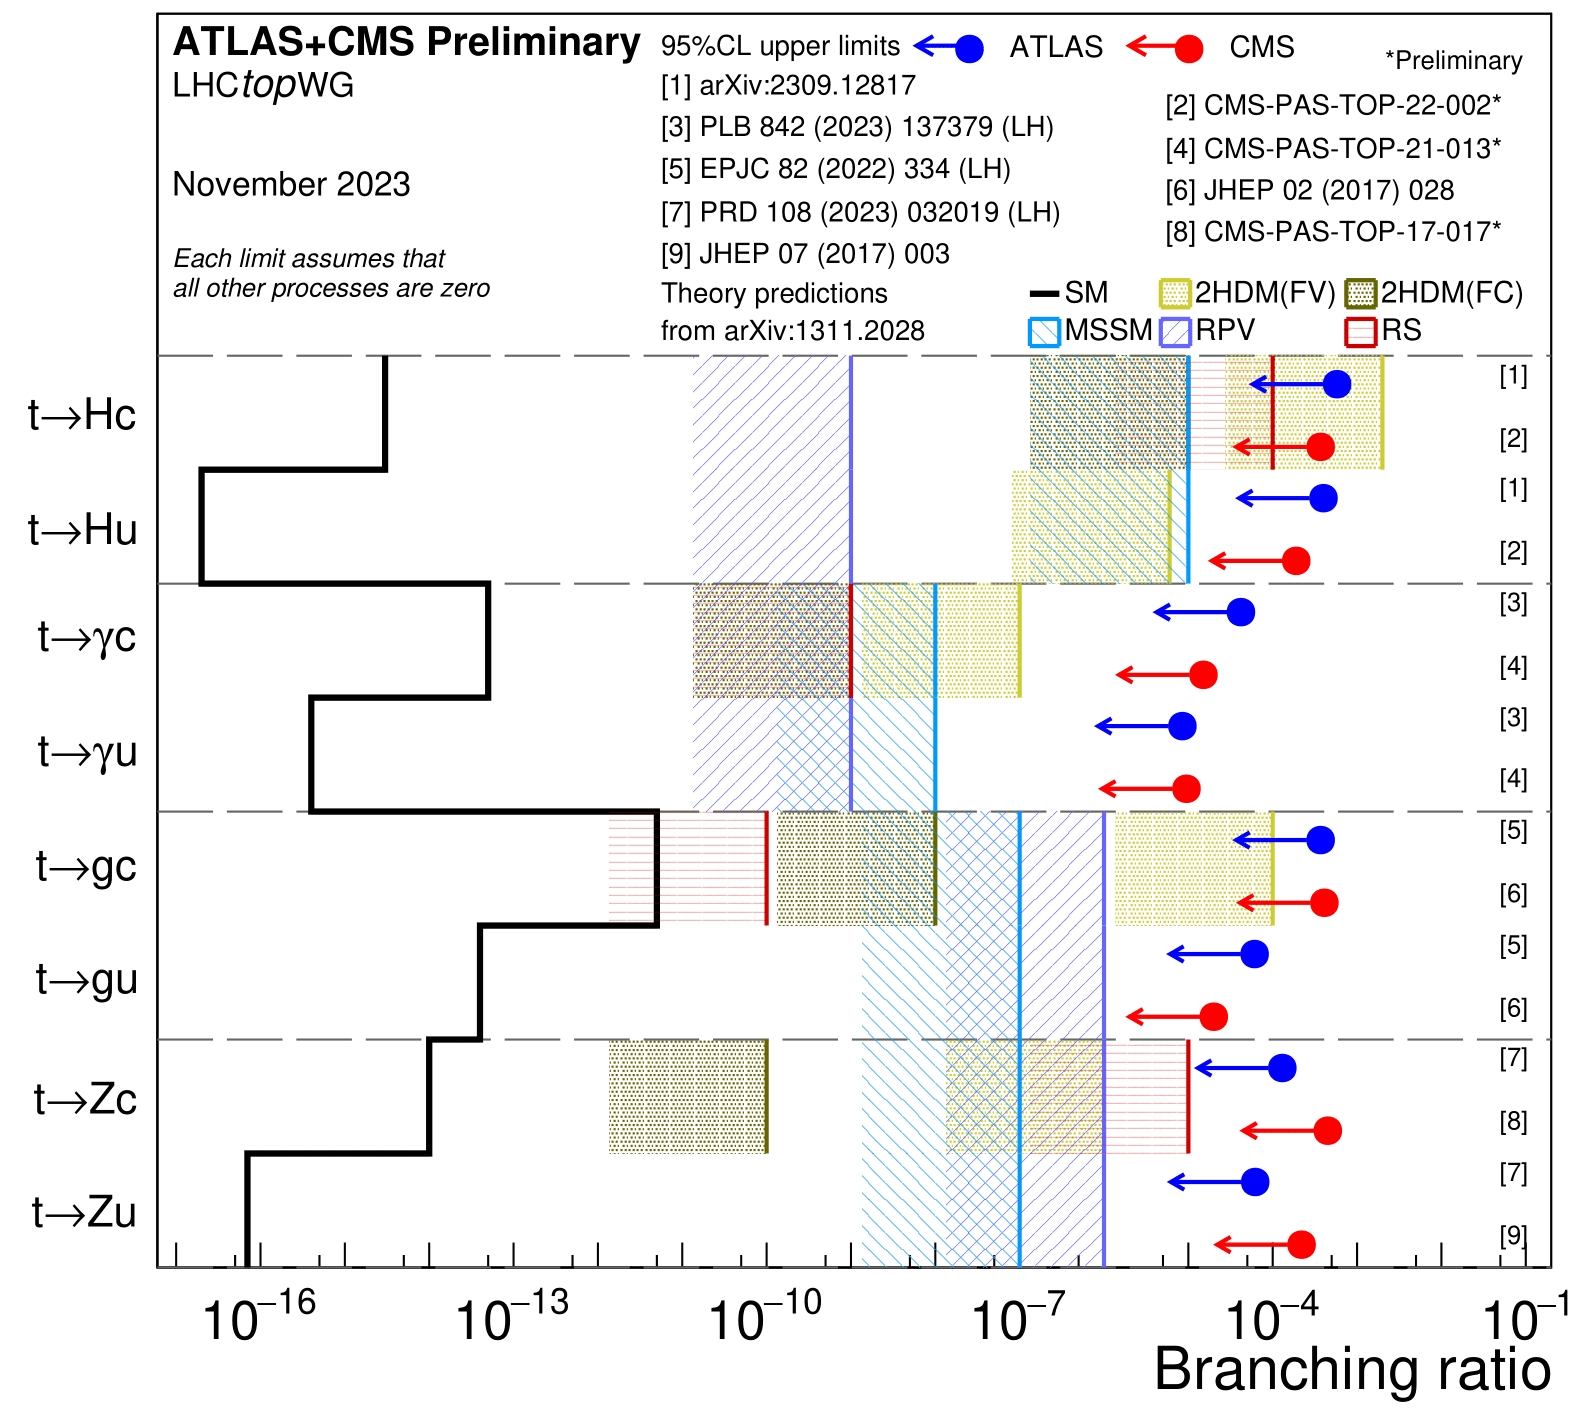
\includegraphics[width=\linewidth]{Presentation_Higgs_performance_meeting19marc_2024/fcnc_summarybsm_nov23.png}
\begin{alertblock}%{Message from the summary plot}
\tiny
\justifying
Several top-FCNC channels are constrained at the \(10^{-5}\)-\(10^{-4}\) level \& FCC-ee as a complementary rare-top machine.
\end{alertblock}
\end{column}
\end{columns}
%\refs{Local public-summary plot included in the analysis package (ATLAS+CMS topWG, Nov.~2023). Updateable with newer public summaries if desired.}
\end{frame}







%----------------------------------------------------------------------------------------
\begin{frame}{Which FCNC modes matter for FCC-ee?}
\begin{columns}[T,totalwidth=\textwidth]
\begin{column}{0.55\textwidth}
\begin{itemize}
\justifying 
\item In the general anomalous-coupling picture one can write vertices \(tqg\), \(tq\gamma\), \(tqZ\), and \(tqH\).
\item For this talk we concentrate on \alert{\(tq\gamma\)} and \alert{\(tqZ\)} because they induce a clean single-top production channel in \(e^+e^-\) collisions.
\item The light quark is taken as \(q=u,c\), and the quoted study-level results are only presented in terms of the branching fractions \(\mathrm{Br}(t\to c\gamma)\) and \(\mathrm{Br}(t\to cZ)\).
\end{itemize}
\end{column}
\begin{column}{0.44\textwidth}
\centering
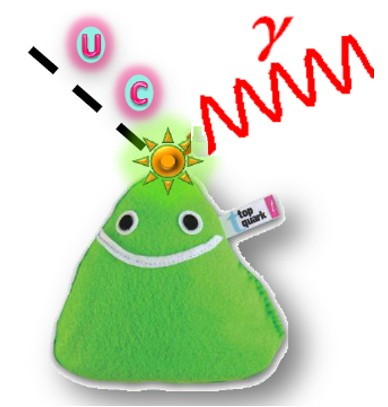
\includegraphics[width=0.60\linewidth]{tqgamma}
\end{column}
\end{columns}
%\refs{Internal draft note and local theory figures.}
\begin{block}{Working focus of the presentation}
\small 
\justifying 
Production-level FCNC in \(e^+e^-\to tq\) followed by standard top decay, analysed in semileptonic and fully hadronic final states.
\end{block}
\end{frame}






%----------------------------------------------------------------------------------------
\begin{frame}{Effective-field-theory \& effective-Lagrangian framework}
\begin{columns}[T,totalwidth=\textwidth]
\begin{column}{\textwidth}
\small
\justifying 
The most general FCNC effective interaction used in the study can be written as
\[
\begin{aligned}
\mathcal{L}_{\mathrm{FCNC}}^{tqX}
= \sum_{q=u,c}\Bigg[
&\frac{g_s}{2m_t}\,\bar q \lambda^a \sigma^{\mu\nu}
(\zeta^L_{qt}P_L+\zeta^R_{qt}P_R)tG^a_{\mu\nu} \\[0.3em]
&-\frac{1}{\sqrt2}\,\bar q(\eta^L_{qt}P_L+\eta^R_{qt}P_R)tH
\\[0.3em]
&-\frac{g_W}{2c_W}\,\bar q\gamma^\mu
(X^L_{qt}P_L+X^R_{qt}P_R)tZ_\mu \\[0.3em] 
&+{\color{blue}\frac{g_W}{4c_Wm_Z}\,\bar q\sigma^{\mu\nu}
(\kappa^L_{qt}P_L+\kappa^R_{qt}P_R)tZ_{\mu\nu}}
\\[0.3em]
&+{\color{red}\frac{e}{2m_t}\,\bar q\sigma^{\mu\nu}
(\lambda^L_{qt}P_L+\lambda^R_{qt}P_R)tA_{\mu\nu}}
\Bigg]+\mathrm{h.c.}
\end{aligned}
\]
\vspace{-0.6em}
\begin{itemize}
\justifying 
\item The analysis sets limits on couplings and then translates them into branching-ratio sensitivities.
\end{itemize}
\end{column}
\begin{tikzpicture}[remember picture,overlay]
\node at ([xshift=4.35cm,yshift=1.65cm]current page.center)
{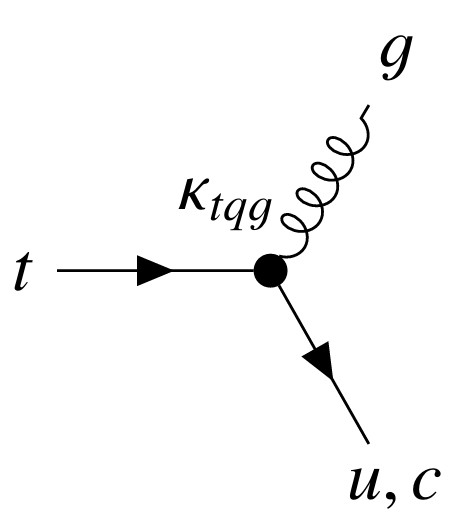
\includegraphics[width=1.8cm]{fcnc1}};
\node at ([xshift=5.95cm,yshift=1.65cm]current page.center)
{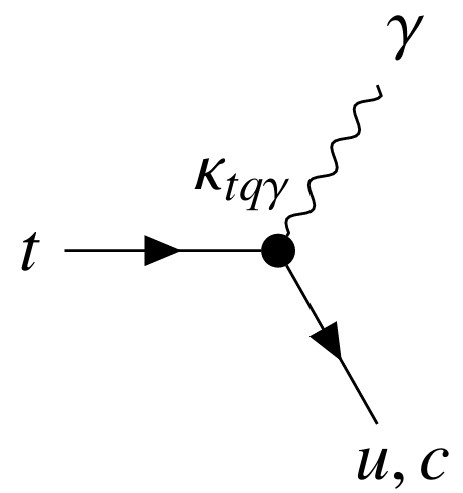
\includegraphics[width=1.8cm]{fcnc2}};

\node at ([xshift=4.35cm,yshift=0.10cm]current page.center)
{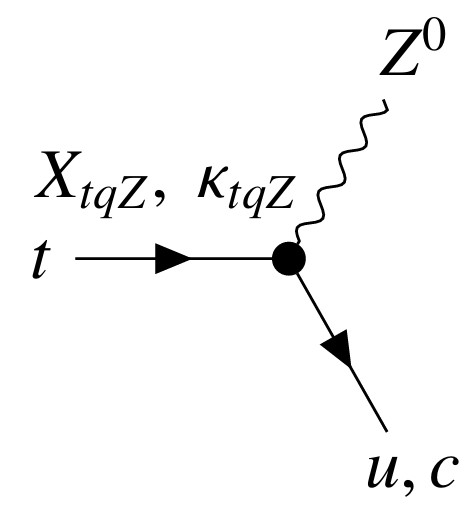
\includegraphics[width=1.8cm]{fcnc3}};
\node at ([xshift=5.95cm,yshift=0.10cm]current page.center)
{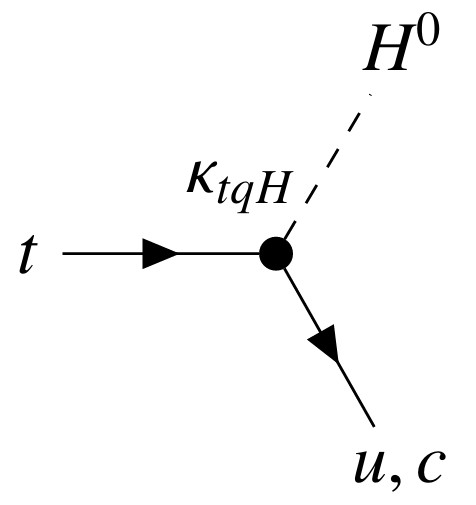
\includegraphics[width=1.8cm]{fcnc4}};
\end{tikzpicture}
\end{columns}
\refs{Aguilar-Saavedra, Nucl. Phys. B812 (2009) 181.}
\end{frame}






%----------------------------------------------------------------------------------------
\begin{frame}{Coupling choices, operator assumptions, and benchmark setup}
\begin{columns}[T,totalwidth=\textwidth]
\begin{column}{0.54\textwidth}
\begin{block}{Assumptions used in the study}
\begin{itemize}
\justifying 
\item One anomalous coupling switched on at a time.
\item Symmetric chiral choice in the benchmark generation:\newline
  \(\lambda^L_{qt}=\lambda^R_{qt}\equiv\lambda_{qt}\),
  \(\kappa^L_{qt}=\kappa^R_{qt}\equiv\kappa_{qt}\).
\item Benchmark signal normalisation generated with representative values \(\lambda_{qt}=0.1\) or \(\kappa_{qt}=0.1\).
\item Limits are finally reported as 95\%~CL sensitivities to \(\mathrm{Br}(t\to c\gamma)\) and \(\mathrm{Br}(t\to cZ)\).
\end{itemize}
\end{block}
\end{column}
\begin{column}{0.42\textwidth}
\begin{block}{Analysis benchmarks}
\centering
\begin{tabular}{@{}lcc@{}}
\toprule
Benchmark & \(\sqrt{s}\) & \(\mathcal{L}_{\mathrm{int}}\) \\
\midrule
Higgs stage & 240 GeV & 5 ab$^{-1}$ \\
Top / EW stage & 365 GeV & 1.5 ab$^{-1}$ \\
\bottomrule
\end{tabular}
\end{block}
\vspace{0.4em}
\begin{tcolorbox}[colback=white,colframe=black!30]
\small
\justifying
Quoted sensitivities are obtained from benchmark signal samples at
\(\sqrt{s}=240\) and \(365\) GeV, and are finally reported as
95\% CL limits on \(\mathrm{Br}(t\to c\gamma)\) and
\(\mathrm{Br}(t\to cZ)\).
\end{tcolorbox}
\end{column}
\end{columns}
%\refs{Internal draft note, theoretical framework and sample definition.}
\end{frame}







%----------------------------------------------------------------------------------------
\begin{frame}{FCC-ee working points for the top-FCNC study: 240 GeV and 365 GeV}
\vspace{-0.30cm}	
\begin{columns}[T,totalwidth=\textwidth]
\begin{column}{0.48\textwidth}
\begin{exampleblock}{\(\sqrt{s}=240\,\mathrm{GeV}\)}
\begin{itemize}
\small
\justifying
\item FCC-ee Higgs-stage working point used in the study.
\item Clean environment for single-top FCNC searches with low hadronic activity.
\item Event kinematics remain closer to threshold, so reconstructed masses, missing energy, and momentum-balance observables provide strong discrimination.
\item Particularly useful for controlling backgrounds and exploiting precise event reconstruction.
\end{itemize}
\end{exampleblock}
\end{column}
		
\begin{column}{0.48\textwidth} 
\begin{alertblock}{\(\sqrt{s}=365\,\mathrm{GeV}\)} 
\begin{itemize} 
\small 
\justifying 
\item FCC-ee top / electroweak working point used in the study.
\item Larger phase space for \(e^+e^- \to tq\), with harder light-jet and reconstructed-top spectra.
\item Stronger kinematic separation between signal and background in several observables.
\item Directly connected to the broader FCC-ee top programme and rare-top sensitivity.
\end{itemize} 
\end{alertblock} 
\end{column} 
		  
\end{columns} 
	
%\vspace{0.1em} 

\begin{block}{Analysis strategy consequence} 
\small 
\justifying 
The same top-FCNC signal hypothesis is tested at both FCC-ee working points, but the optimal event selections differ because the signal and background kinematics evolve significantly from the 240 GeV Higgs stage to the 365 GeV top / electroweak stage.
\end{block}
%\refs{Internal draft benchmark choice and event-selection sections.}
\end{frame}
%----------------------------------------------------------------------------------------






%----------------------------------------------------------------------------------------
\section{{\color{white}Signal process and analysis design}}


\begin{frame}{Signal process at FCC-ee: single-top production from \texorpdfstring{$tq\gamma$ and $tqZ$}{tqgamma and tqZ}}
\begin{columns}[T,totalwidth=\textwidth]
%\begin{column}{0.48\textwidth}
%\centering
%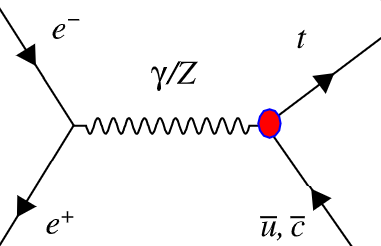
\includegraphics[width=\linewidth]{Presentation_Higgs_performance_meeting19marc_2024/feyn1_SM_ee.png}
%\vspace{0.4em}
%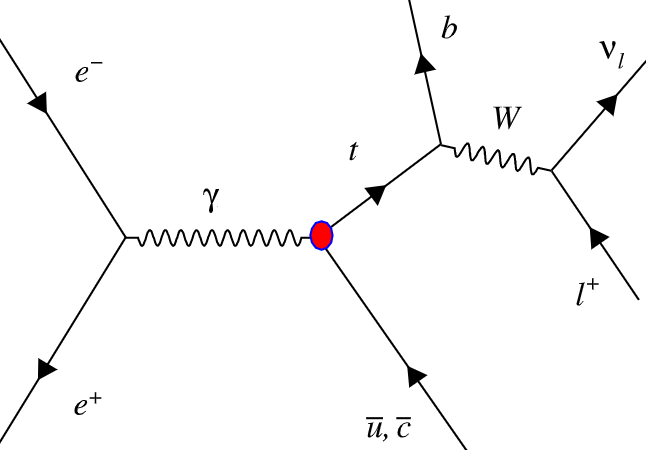
\includegraphics[width=0.92\linewidth]{Presentation_Higgs_performance_meeting19marc_2024/Feyn.png}
%\end{column}
\begin{column}{\textwidth}
\begin{itemize}
\justifying 
\item The FCNC interaction appears at the \alert{production level}: \(e^+e^-\to \gamma/Z \to tq\) and charge-conjugate channels.
\item The top quark then decays dominantly through the Standard Model mode \(t\to Wb\).
\item Two analysis paths are considered:
\begin{itemize}
\justifying 
\item semileptonic: \(\ell\nu b + j\),
\item fully hadronic: \(jjb + j\).
\end{itemize}
\justifying 
\item The light jet from the FCNC vertex is typically energetic and becomes a key discriminant.
\end{itemize}
\end{column}
\end{columns}
%\refs{Internal note signal definition and local signal-process figures.}
\end{frame}






%----------------------------------------------------------------------------------------
\begin{frame}{Analysis workflow at a glance}
\centering
\resizebox{0.96\textwidth}{!}{%
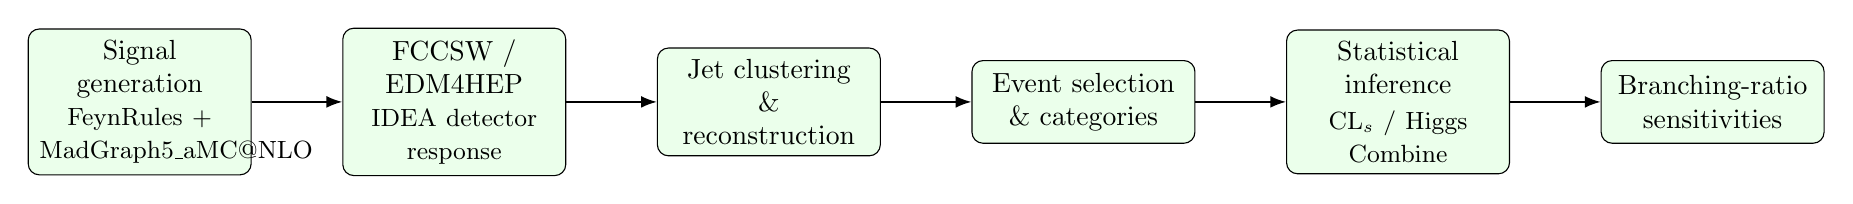
\begin{tikzpicture}[>=Latex,node distance=1.15cm]
\tikzset{
				stepbox/.style={
					draw,
					rounded corners,
					fill=green!8,
					text width=2.55cm,
					minimum height=1.05cm,
					align=center,
					inner sep=4pt
				}
			}
			\node[stepbox] (gen) {Signal generation\\[0.1em]\small FeynRules +\\ MadGraph5\_aMC@NLO};
			\node[stepbox,right=of gen] (sim) {FCCSW / EDM4HEP\\[0.1em]\small IDEA detector\\ response};
			\node[stepbox,right=of sim] (rec) {Jet clustering\\ \& reconstruction};
			\node[stepbox,right=of rec] (sel) {Event selection\\ \& categories};
			\node[stepbox,right=of sel] (stat) {Statistical inference\\[0.1em]\small CL$_s$ / Higgs Combine};
			\node[stepbox,right=of stat] (br) {Branching-ratio\\ sensitivities};
			
			\draw[->,semithick] (gen) -- (sim);
			\draw[->,semithick] (sim) -- (rec);
			\draw[->,semithick] (rec) -- (sel);
			\draw[->,semithick] (sel) -- (stat);
			\draw[->,semithick] (stat) -- (br);
\end{tikzpicture}%
}
\vspace{0.5cm}
	
\begin{block}{Core logic}
\small
\justifying
Production-level FCNC signal samples are propagated through the official FCC software chain, reconstructed with the chosen jet algorithm, separated from backgrounds through channel-dependent selections, and finally interpreted as sensitivities to \(\mathrm{Br}(t\to c\gamma)\) and \(\mathrm{Br}(t\to cZ)\). 
\end{block}
%\refs{Internal draft note; local workflow concept adapted to AGH style.}
\end{frame}
%----------------------------------------------------------------------------------------




%----------------------------------------------------------------------------------------
\begin{frame}{Detector and simulation framework: FCCSW / IDEA / signal samples}
\begin{columns}[T,totalwidth=\textwidth]
\begin{column}{0.56\textwidth}
\begin{itemize}
\justifying 
\item The analysis is performed in the \alert{official FCC analysis framework} with Delphes-based IDEA detector response [{\color{blue}2502.21223 [physics.ins-det]}].
\item Official signal samples are generated with \texttt{MadGraph5\_aMC@NLO} using the FCNC effective model implemented through \texttt{FeynRules}/UFO.
\item Flavour-tagging WP: \(\epsilon_b=80\%\), \(\epsilon_c=10\%\).
\item Jet reconstruction algorithm: ee-kT Durham + E-scheme recombination.
\end{itemize}
\end{column}
\begin{column}{0.39\textwidth}
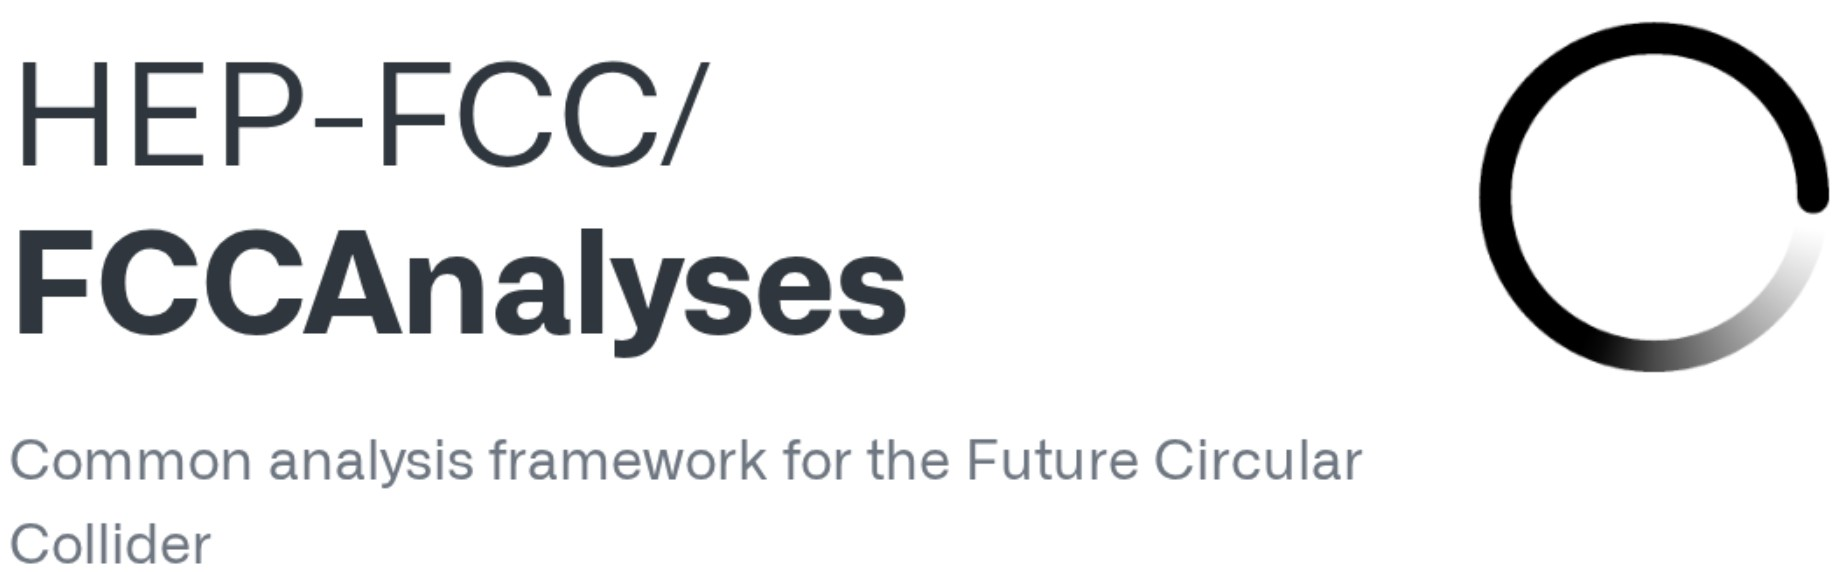
\includegraphics[width=\linewidth]{FCCanalysis.jpg}
\footnotesize
{\color{red}https://hep-fcc.github.io/FCCAnalyses/}
\end{column}
\end{columns}
\begin{block}{FCCAnalyses framework}
\small
\justifying
\texttt{FCCAnalyses} is the standard FCC analysis environment for detector-level phenomenology studies. It allows one to process EDM4HEP samples, reconstruct physics objects, define observables and selections, and produce the histograms and reduced ntuples used in physics sensitivity projections.
\end{block}
\end{frame}






%----------------------------------------------------------------------------------------
\begin{frame}{Event topology: semileptonic channel}
\begin{columns}[T,totalwidth=\textwidth]
%\documentclass[tikz,border=2pt]{standalone}
\begin{column}{0.40\textwidth}
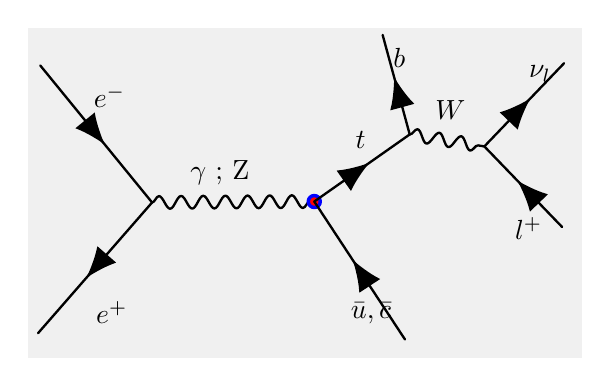
\begin{tikzpicture}[
		x=0.40cm,
		y=0.40cm,
		line cap=round,
		line join=round,
		fermion/.style={
			draw=black,
			line width=0.85pt,
			postaction={decorate},
			decoration={
				markings,
				mark=at position 0.58 with {\arrow{Latex[length=4.0mm,width=3.2mm]}}
			}
		},
		photon/.style={
			draw=black,
			line width=0.85pt,
			decorate,
			decoration={snake,amplitude=2.3pt,segment length=8.0pt}
		}
		]
		
		% background
		\fill[gray!12] (-3.95,-4.95) rectangle (13.65,5.55);
		
		% key vertices
		\coordinate (L)  at (0.00, 0.00);
		\coordinate (C)  at (5.15, 0.03);
		\coordinate (T)  at (8.18, 2.16);
		\coordinate (Wv) at (10.55, 1.78);
		
		% external endpoints
		\coordinate (em) at (-3.55, 4.35);
		\coordinate (ep) at (-3.62,-4.15);
		\coordinate (q)  at (8.03,-4.35);
		\coordinate (b)  at (7.32, 5.32);
		\coordinate (nu) at (13.08, 4.42);
		\coordinate (lp) at (13.02,-0.78);
		
		% left incoming legs
		\draw[fermion] (em) -- (L);
		\draw[fermion] (L) -- (ep);
		
		% photon
		\draw[photon] (L) -- (C);
		
		% anomalous FCNC vertex
		\filldraw[fill=red,draw=blue,line width=1.25pt] (C) circle (0.19);
		
		% top and anti-u,c lines
		\draw[fermion] (C) -- (T);
		\draw[fermion] (q) -- (C);
		
		% top decay
		\draw[fermion] (T) -- (b);
		\draw[photon]  (T) -- (Wv);
		
		% W decay products
		\draw[fermion] (Wv) -- (nu);
		\draw[fermion] (lp) -- (Wv);
		
		% labels
		\node at (-1.35, 3.35) {$e^{-}$};
		\node at (-1.28,-3.48) {$e^{+}$};
		
		\node at (2.15, 0.95) {$\gamma$ ; Z};
		
		\node at (6.62, 1.98) {$t$};
		\node at (6.95,-3.52) {$\bar u,\bar c$};
		
		\node at (7.85, 4.58) {$b$};
		\node at (9.47, 2.92) {$W$};
		
		\node at (12.32, 4.08) {$\nu_l$};
		\node at (11.96,-0.82) {$l^{+}$};
\end{tikzpicture}
\end{column}
\begin{column}{0.40\textwidth}
\begin{block}{Signal signature}
\begin{itemize}
\justifying 
\item exactly one isolated charged lepton \((e\;\text{or}\;\mu)\),
\item missing energy from the neutrino,
\item exactly two exclusive jets,
\item one b-tagged jet and one energetic light jet.
\item Baseline selection: \(p_{\ell,j}>15\,\mathrm{GeV}\), \(\theta_{\ell,j}>13^\circ\). 
\end{itemize}
\end{block}
\end{column}
\end{columns}
\vspace{0.5cm}
\begin{itemize}
\justifying 
\item Electron and muon channels are analysed separately and later statistically combined.
\item The reconstructed top mass, W mass, jet momenta, missing energy and angular observables provide the main discrimination power.
\end{itemize}
%\refs{Internal note, leptonic-channel definition; local semileptonic topology figure.}
\end{frame}





%----------------------------------------------------------------------------------------
\begin{frame}{Event topology: fully hadronic channel}
\begin{columns}[T,totalwidth=\textwidth]
\begin{column}{0.40\textwidth}
	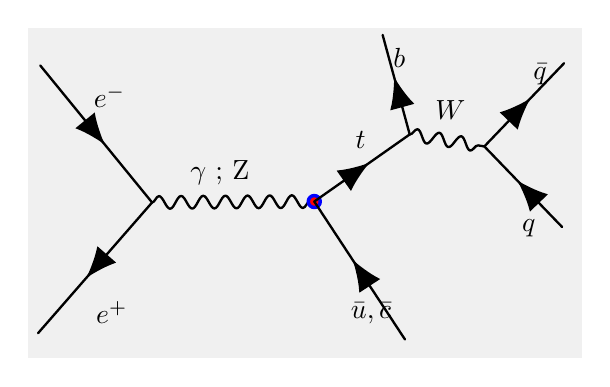
\begin{tikzpicture}[
		x=0.40cm,
		y=0.40cm,
		line cap=round,
		line join=round,
		fermion/.style={
			draw=black,
			line width=0.85pt,
			postaction={decorate},
			decoration={
				markings,
				mark=at position 0.58 with {\arrow{Latex[length=4.0mm,width=3.2mm]}}
			}
		},
		photon/.style={
			draw=black,
			line width=0.85pt,
			decorate,
			decoration={snake,amplitude=2.3pt,segment length=8.0pt}
		}
		]
		
		% background
		\fill[gray!12] (-3.95,-4.95) rectangle (13.65,5.55);
		
		% key vertices
		\coordinate (L)  at (0.00, 0.00);
		\coordinate (C)  at (5.15, 0.03);
		\coordinate (T)  at (8.18, 2.16);
		\coordinate (Wv) at (10.55, 1.78);
		
		% external endpoints
		\coordinate (em) at (-3.55, 4.35);
		\coordinate (ep) at (-3.62,-4.15);
		\coordinate (q)  at (8.03,-4.35);
		\coordinate (b)  at (7.32, 5.32);
		\coordinate (nu) at (13.08, 4.42);
		\coordinate (lp) at (13.02,-0.78);
		
		% left incoming legs
		\draw[fermion] (em) -- (L);
		\draw[fermion] (L) -- (ep);
		
		% photon
		\draw[photon] (L) -- (C);
		
		% anomalous FCNC vertex
		\filldraw[fill=red,draw=blue,line width=1.25pt] (C) circle (0.19);
		
		% top and anti-u,c lines
		\draw[fermion] (C) -- (T);
		\draw[fermion] (q) -- (C);
		
		% top decay
		\draw[fermion] (T) -- (b);
		\draw[photon]  (T) -- (Wv);
		
		% W decay products
		\draw[fermion] (Wv) -- (nu);
		\draw[fermion] (lp) -- (Wv);
		
		% labels
		\node at (-1.35, 3.35) {$e^{-}$};
		\node at (-1.28,-3.48) {$e^{+}$};
		
		\node at (2.15, 0.95) {$\gamma$ ; Z};
		
		\node at (6.62, 1.98) {$t$};
		\node at (6.95,-3.52) {$\bar u,\bar c$};
		
		\node at (7.85, 4.58) {$b$};
		\node at (9.47, 2.92) {$W$};
		
		\node at (12.32, 4.08) {$\bar q$};
		\node at (11.96,-0.82) {$q$};
	\end{tikzpicture}
\end{column}
\begin{column}{0.40\textwidth}
\begin{block}{Signal signature}
\begin{itemize}
\justifying 
\item exactly four exclusive jets,
\item one energetic light jet from the FCNC vertex,
\item one or two b-tagged jets depending on category,
\item low missing energy, since the final state is fully visible.
\item Baseline selection: \(p_{j}>20\,\mathrm{GeV}\),  \(\theta_j>13^\circ\). 
\end{itemize}
\end{block}
\end{column}
\end{columns}
\vspace{0.5cm}
\begin{itemize}
\justifying 
\item The price of larger branching fraction is stronger combinatorics and a much larger \(WW\)-like background.
\item The analysis therefore uses dedicated category logic, \(\chi^2\)-based assignment and fake-W rejection.
\end{itemize}
%\refs{Internal note, fully hadronic analysis section; local hadronic topology figure.}
\end{frame}










%----------------------------------------------------------------------------------------
\begin{frame}{Main background processes at 240 and 365 GeV}
\vspace{-0.4cm}
\begin{columns}[T,totalwidth=\textwidth]
\begin{column}{0.48\textwidth}
\begin{block}{\(\sqrt{s}=240~\mathrm{GeV}\)}
\small
\begin{itemize}
					\item \(e^+e^- \to ZH\) \hfill \(202~\mathrm{fb}\)
					\item \(e^+e^- \to W^+W^-\) \hfill \(16439~\mathrm{fb}\)
					\item \(e^+e^- \to ZZ\) \hfill \(1360~\mathrm{fb}\)
					\item \(e\gamma \to tb\nu\) \hfill \(0.01~\mathrm{fb}\)
					\item \(e\gamma \to Zbb\)  \hfill \(455~\mathrm{fb}\)
					\item \(e\gamma \to Zqq\)  \hfill \(1635~\mathrm{fb}\)
\end{itemize}
\end{block}
\begin{alertblock}{Key point at 240 GeV}
\small
\justifying
The dominant irreducible background is \(W^+W^-\), with additional contributions from
\(ZZ\), \(ZH\), and \(\gamma e\)-initiated processes. No \(t\bar t\) background is present at this energy.
\end{alertblock}
\end{column}
\begin{column}{0.48\textwidth}
\begin{block}{\(\sqrt{s}=365~\mathrm{GeV}\)}
\small
\begin{itemize}
					\item \(e^+e^- \to ZH\) \hfill \(117~\mathrm{fb}\)
					\item \(e^+e^- \to W^+W^-\) \hfill \(10717~\mathrm{fb}\)
					\item \(e^+e^- \to ZZ\) \hfill \(643~\mathrm{fb}\)
					\item \(e\gamma \to tb\nu\) \hfill \(0.22~\mathrm{fb}\)
					\item \(e\gamma \to Zbb\) \hfill \(615~\mathrm{fb}\)
					\item \(e^+e^- \to t\bar t\) \hfill \(800~\mathrm{fb}\)
                    \item \(e^+e^- \to tbjj\) \hfill \(5.98~\mathrm{fb}\)
\end{itemize}
\end{block}
\begin{alertblock}{Key point at 365 GeV}
\small
\justifying
In addition to diboson and \(ZH\) production, the analysis must also contend with genuine
top backgrounds, especially \(t\bar t\) and single-top-like contributions above threshold.
\end{alertblock}
\end{column}
\end{columns}
%\vspace{0.2cm}
%\begin{tcolorbox}[colback=white,colframe=black!30]
%\small
%\justifying
%These are the inclusive benchmark cross sections before any event selection. The analysis strategy is therefore driven by strong rejection of diboson backgrounds at 240 GeV, while at 365 GeV one must additionally separate the FCNC signal from Standard-Model top production.
%\end{tcolorbox}
%\refs{Internal draft note, Table I: MC samples and benchmark cross sections at 240 and 365 GeV.}
\end{frame}
%----------------------------------------------------------------------------------------







%----------------------------------------------------------------------------------------
\begin{frame}{Jet clustering and reconstruction strategy}
\begin{columns}[T,totalwidth=\textwidth]
\begin{column}{0.45\textwidth}
\centering
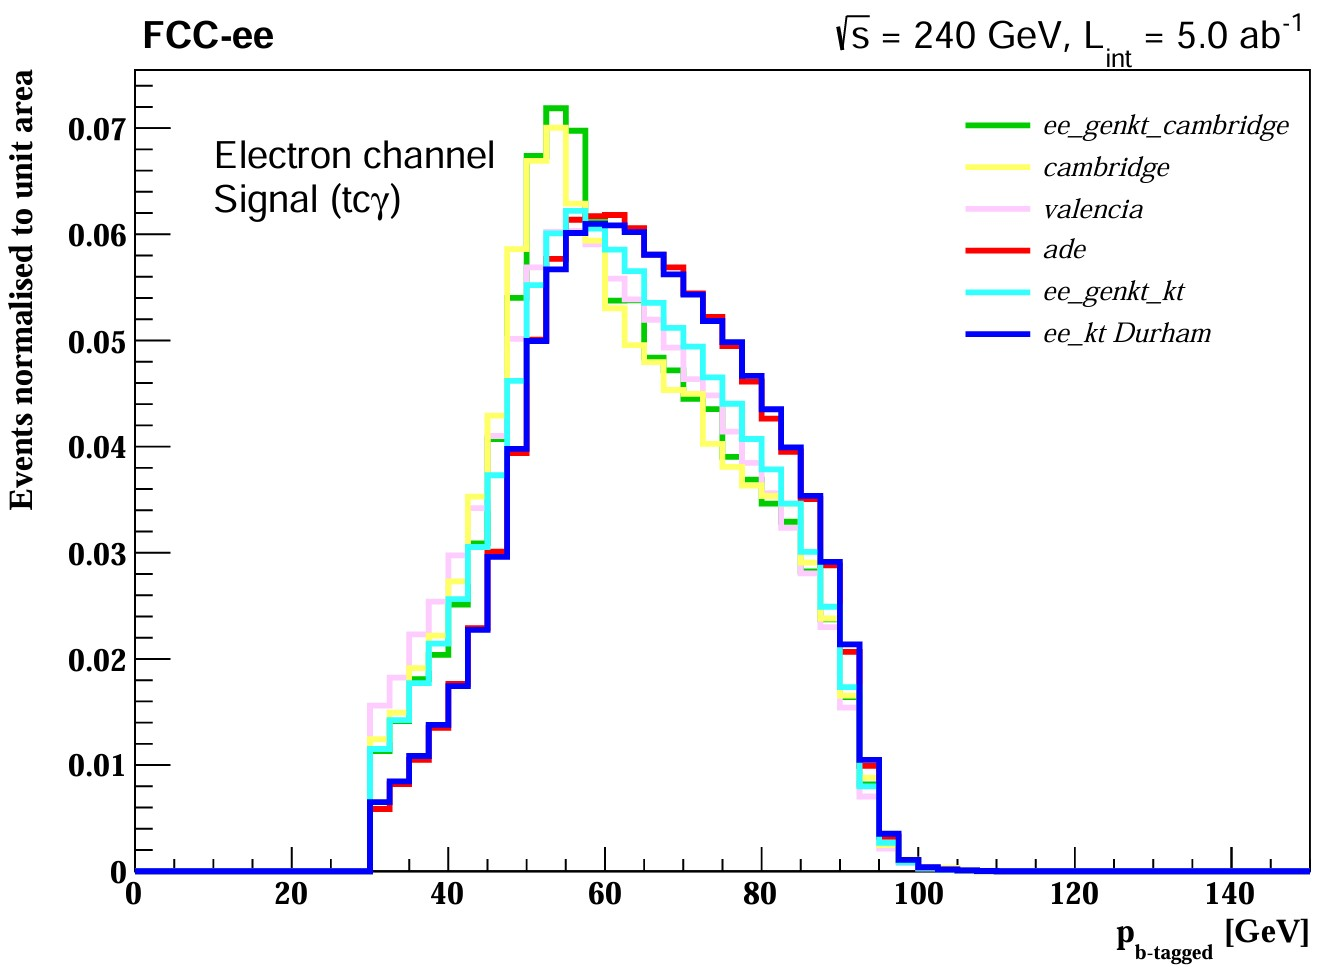
\includegraphics[width=\linewidth]{algorithms_1.jpg}
\end{column}
\begin{column}{0.45\textwidth}
\centering
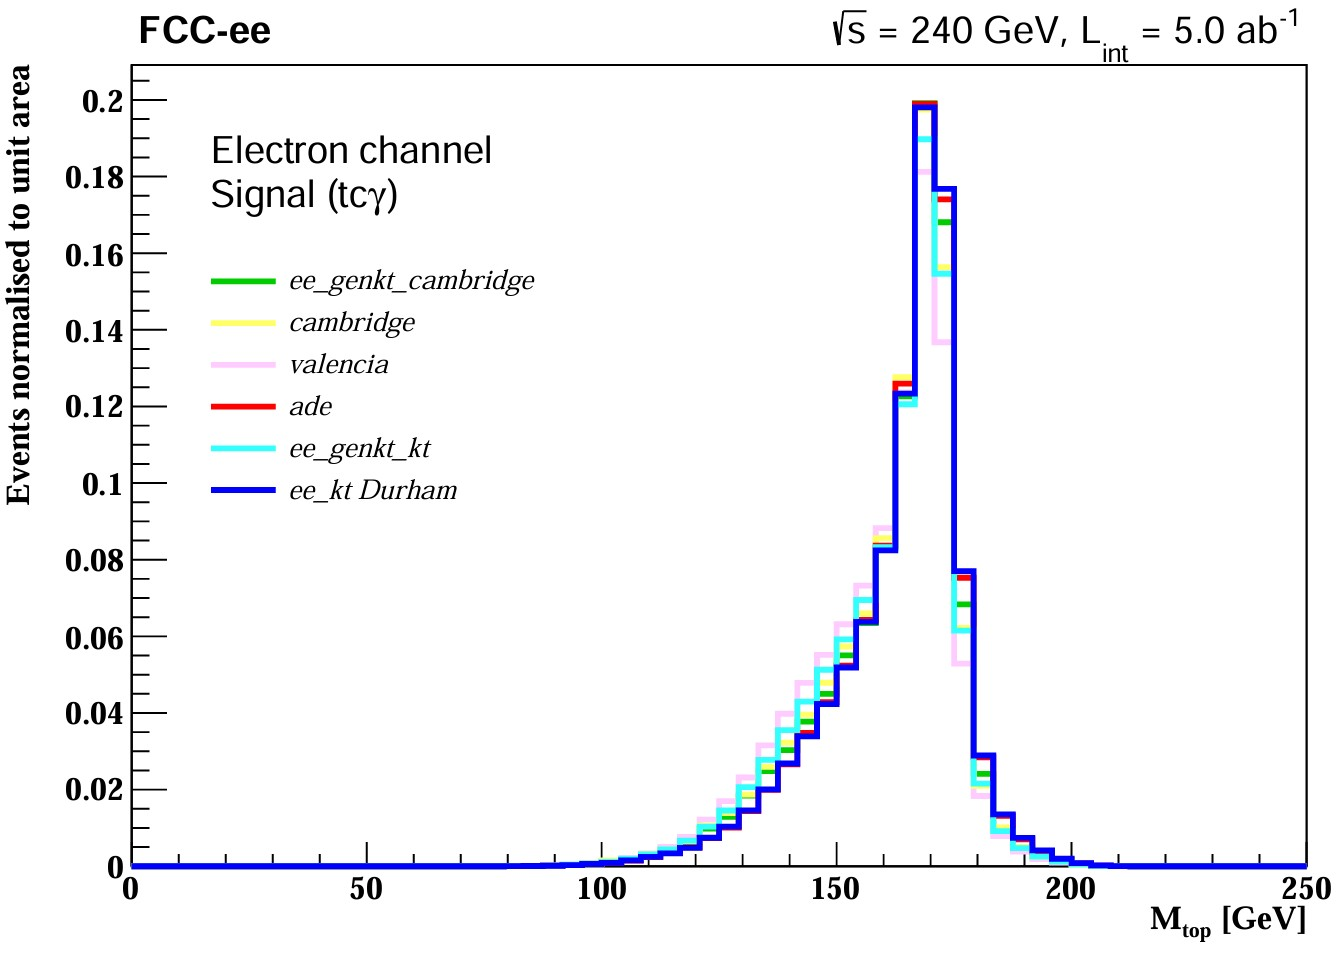
\includegraphics[width=\linewidth]{algorithms_2.jpg}
\end{column}
\end{columns}
\vspace{0.4em}
\begin{itemize}
\justifying 
\item Several official jet algorithms were tested; the final analysis adopts the \alert{ee-kT Durham} clustering with the \alert{E-scheme} recombination.
\item Exclusive \(N_{\mathrm{jet}}=2\) and \(N_{\mathrm{jet}}=4\) modes are used for the semileptonic and hadronic analyses, respectively.
\item The choice is driven by reconstructed-top stability and by the behaviour of the b-jet candidate momentum.
\end{itemize}
%\refs{Internal jet-algorithm study and local comparison figures.}
\end{frame}







%----------------------------------------------------------------------------------------
\begin{frame}{Semileptonic reconstruction and discriminating observables}
\begin{columns}[T,totalwidth=\textwidth]
\begin{column}{0.47\textwidth}
\centering

\includegraphics[width=\linewidth]{Wmass-240GeV-leptonic.jpg}
\end{column}
\begin{column}{0.47\textwidth}
\centering

\includegraphics[width=\linewidth]{topmass-240GeV-leptonic.jpg}
\end{column}
\end{columns}
\vspace{0.2em}
\begin{itemize}
\justifying 
\item The strongest semileptonic discriminants are the reconstructed \(M_{\mathrm{top}}\), \(M_W\), \(p_b\), \(p_{\mathrm{light\,jet}}\), missing energy, \(\Delta R(\ell,b)\), and global activity variables such as \(H_T\).
\item The plots shown are representative for the electron channel at 240~GeV; the same logic is applied at 365~GeV and in the muon channel.
\end{itemize}
%\refs{Internal draft note, leptonic reconstruction figures and Plots-240 package.}
\end{frame}






%----------------------------------------------------------------------------------------
\begin{frame}{Fully hadronic reconstruction and discriminating observables}
\begin{columns}[T,totalwidth=\textwidth]
\begin{column}{0.47\textwidth}
\centering

\includegraphics[width=\linewidth]{Wmass-full-240GeV.jpg}
\end{column}
\begin{column}{0.47\textwidth}
\centering

\includegraphics[width=\linewidth]{topmass-full-240GeV.jpg}
\end{column}
\end{columns}
\vspace{0.2em}
\begin{itemize}
\justifying 
\item The hadronic analysis reconstructs the signal candidate with a \(\chi^2\)-type assignment to the \(W\) and top hypotheses.
\item The fake-W mass, missing energy, angular separations and light-jet / b-jet momentum ratios are crucial for suppressing the overwhelming \(WW\) background.
\end{itemize}
%\refs{Internal draft note, fully hadronic reconstruction figures.}
\end{frame}







%----------------------------------------------------------------------------------------
\begin{frame}{Light-jet momentum as a discriminating observable}
\begin{columns}[T,totalwidth=\textwidth]
\begin{column}{0.47\textwidth}
\centering

\includegraphics[width=\linewidth]{plightjet-240GeV-leptonic.jpg}
\end{column}
\begin{column}{0.47\textwidth}
\centering

\includegraphics[width=\linewidth]{plightjet-full-240GeV.jpg}
\end{column}
\end{columns}
\vspace{0.2em}
\begin{itemize}
\justifying
\item The light jet originates directly from the FCNC production vertex \(e^+e^- \to tq\), so it tends to be relatively energetic and carries useful kinematic information on the signal topology.
\item Its momentum spectrum differs from the dominant Standard Model backgrounds, where jets are more often produced through diboson decays or other sources. 
\end{itemize}
%\refs{Internal draft note, fully hadronic reconstruction figures.}
\end{frame}









%----------------------------------------------------------------------------------------
\begin{frame}{Event selection / cut-flow / category logic}
\begin{columns}[T,totalwidth=\textwidth]
\begin{column}{0.52\textwidth}
\small
\begin{block}{Representative selection windows}
\begin{itemize}
\justifying
\item \textbf{Leptonic 240 GeV:} \(140<M_{\rm top}<190\) GeV, \(70<M_W<90\) GeV, \(p_b>40\) GeV, \(p_{\ell}>20\) GeV, \(E_T^{\rm miss}>30\) GeV, \(H_T>190\) GeV.
\item \textbf{Leptonic 365 GeV:} same mass windows, but harder light-jet and event-activity requirements, e.g. \(p_{\rm light}>120\) GeV and \(H_T>300\) GeV.
\item \textbf{Hadronic 240\&365 GeV:} category-dependent cuts on \(M_{\rm top}\), \(M_W\), fake-W mass, low missing energy, and angular separations among the jets.
\end{itemize}
\end{block}
\end{column}
\begin{column}{0.45\textwidth}
\small
\begin{tabular}{@{}lcc@{}}
\toprule
Channel & signal [fb] & total bkg [fb] \\
\midrule
LDC, 240 GeV & 1.37 (\(tc\gamma\)) & 0.457 \\
LDC, 365 GeV & 1.96 (\(tc\gamma\)) & 1.140 \\
HDC, 240 GeV & 6.61 (\(tc\gamma\)) & 299.59 \\
HDC, 365 GeV & 14.50 (\(tc\gamma\)) & 66.02 \\
\bottomrule
\end{tabular}
\vspace{0.4em}
\begin{tcolorbox}[colback=white,colframe=black!30]
\small
\justifying
Main message: the fully hadronic channel starts from a harsher background environment but still provides useful complementary sensitivity once topology-driven selections are applied.
\end{tcolorbox}
\end{column}
\end{columns}
%\refs{Signal and background cross sections after final selections extracted from the internal draft note.}
\end{frame}






%----------------------------------------------------------------------------------------
\begin{frame}{Statistical procedure and limit extraction}
\begin{columns}[T,totalwidth=\textwidth]
\begin{column}{0.55\textwidth}
\begin{itemize}
\justifying
\item The final sensitivities are obtained with the standard \alert{CL$_s$} approach using the \alert{Higgs Combine} toolkit.
\item Limits are first extracted channel by channel:
\begin{itemize}
\justifying
\item electron and muon semileptonic channels,
\item fully hadronic channel,
\item 240 GeV and 365 GeV benchmarks.
\end{itemize}
\item The results are then statistically combined across energies and channels.
\item Finally, the coupling limits are translated into limits on the branching ratios \(\mathrm{Br}(t\to c\gamma)\) and \(\mathrm{Br}(t\to cZ)\).
\end{itemize}
%\[
%CL_s = \frac{CL_{s+b}}{CL_b}
%\]
\end{column}
\begin{column}{0.40\textwidth}
\centering
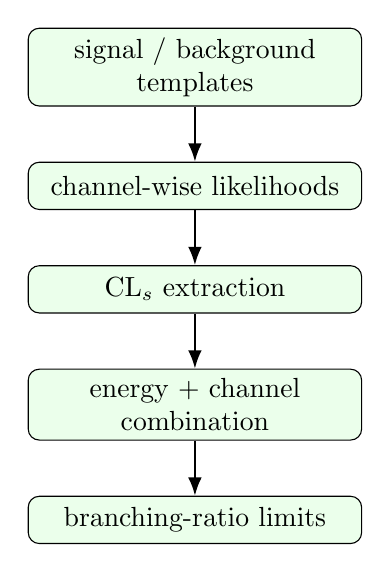
\begin{tikzpicture}[>=Latex,node distance=0.7cm]
	\tikzstyle{box}=[draw,rounded corners,fill=green!8,text width=4.0cm,minimum height=0.6cm,align=center]
	\node[box] (a) {signal / background templates};
	\node[box,below=of a] (b) {channel-wise likelihoods};
	\node[box,below=of b] (c) {CL$_s$ extraction};
	\node[box,below=of c] (d) {energy + channel combination};
	\node[box,below=of d] (e) {branching-ratio limits};
	\draw[->,thick] (a)--(b);
	\draw[->,thick] (b)--(c);
	\draw[->,thick] (c)--(d);
	\draw[->,thick] (d)--(e);
\end{tikzpicture}
\end{column}
\end{columns}
\vspace{0.2cm}
\refs{Higgs Combine toolkit: https://github.com/cms-analysis/HiggsAnalysis-CombinedLimit}
\end{frame}






%----------------------------------------------------------------------------------------
\section{{\color{white}Sensitivity estimation}}

\begin{frame}{Results at 240 GeV and 365 GeV}
\begin{columns}[T,totalwidth=\textwidth]
\begin{column}{0.48\textwidth}
\begin{block}{Semileptonic analysis}
\centering
\begin{tabular}{@{}lcc@{}}
\toprule
Channel & \(\mathrm{Br}(t\to c\gamma)\) & \(\mathrm{Br}(t\to cZ)\) \\
\midrule
\multicolumn{3}{c}{\(\sqrt{s}=240\) GeV, \(5\,\mathrm{ab}^{-1}\)} \\
\midrule
Electron & $9.60\times 10^{-5}$ & $3.53\times 10^{-5}$ \\
Muon & $6.29\times 10^{-5}$ & $2.31\times 10^{-5}$ \\
\midrule
\multicolumn{3}{c}{\(\sqrt{s}=365\) GeV, \(1.5\,\mathrm{ab}^{-1}\)} \\
\midrule
Electron & $1.65\times 10^{-4}$ & $6.96\times 10^{-5}$ \\
Muon & $1.47\times 10^{-4}$ & $6.19\times 10^{-5}$ \\
\bottomrule
\end{tabular}
\end{block}
\end{column}
\begin{column}{0.48\textwidth}
\begin{alertblock}{Fully hadronic analysis}
\centering
\begin{tabular}{@{}lcc@{}}
\toprule
Channel & \(\mathrm{Br}(t\to c\gamma)\) & \(\mathrm{Br}(t\to cZ)\) \\
\midrule
\(240\) GeV & $1.98\times 10^{-4}$ & $1.01\times 10^{-4}$ \\
\(365\) GeV & $8.45\times 10^{-5}$ & $3.70\times 10^{-5}$ \\
\bottomrule
\end{tabular}
\end{alertblock}
\vspace{0.45em}
\begin{tcolorbox}[colback=white,colframe=black!30]
\small
\justifying
Best single-channel sensitivity in the current study comes from the \alert{combined semileptonic analysis}, while the hadronic channel provides a meaningful complementary constraint.
\end{tcolorbox}
\end{column}
\end{columns}
\vspace{0.2cm}
\refs{{\color{red}Top FCNC analysis note: FCC Physics and Experiments:  https://repository.cern/records/avxy7-mtz86}.}
\end{frame}






%----------------------------------------------------------------------------------------
\begin{frame}{Combined sensitivities and comparison with other experiments}
\begin{columns}[T,totalwidth=\textwidth]
\begin{column}{0.99\textwidth}
\begin{block}{Combined sensitivities}
\centering
\small
%\footnotesize
\begin{tabular}{@{}>{\raggedright\arraybackslash}p{0.56\linewidth}
>{\centering\arraybackslash}p{0.18\linewidth}
>{\centering\arraybackslash}p{0.18\linewidth}@{}}
\toprule
Combination & $\mathrm{Br}(t\to c\gamma)$ & $\mathrm{Br}(t\to cZ)$ \\
\midrule
Leptonic: energies + channels & $1.99\times10^{-5}$ & $8.19\times10^{-6}$ \\
Hadronic: energies combined   & $7.65\times10^{-5}$ & $3.28\times10^{-5}$ \\
\bottomrule
\end{tabular}
\end{block}
\end{column}
%\begin{column}{0.62\textwidth}
%\begin{columns}[T,totalwidth=\linewidth]
%\begin{column}{0.49\linewidth}
%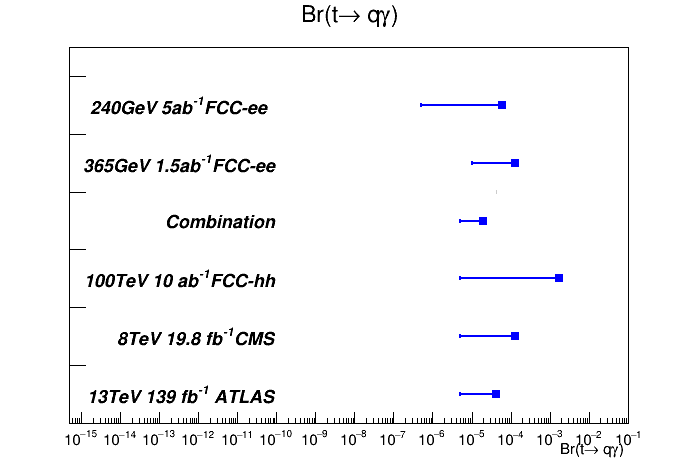
\includegraphics[width=\linewidth]{Presentation_Higgs_performance_meeting19marc_2024/tqa_compare2.png}
%\end{column}
%\begin{column}{0.49\linewidth}
%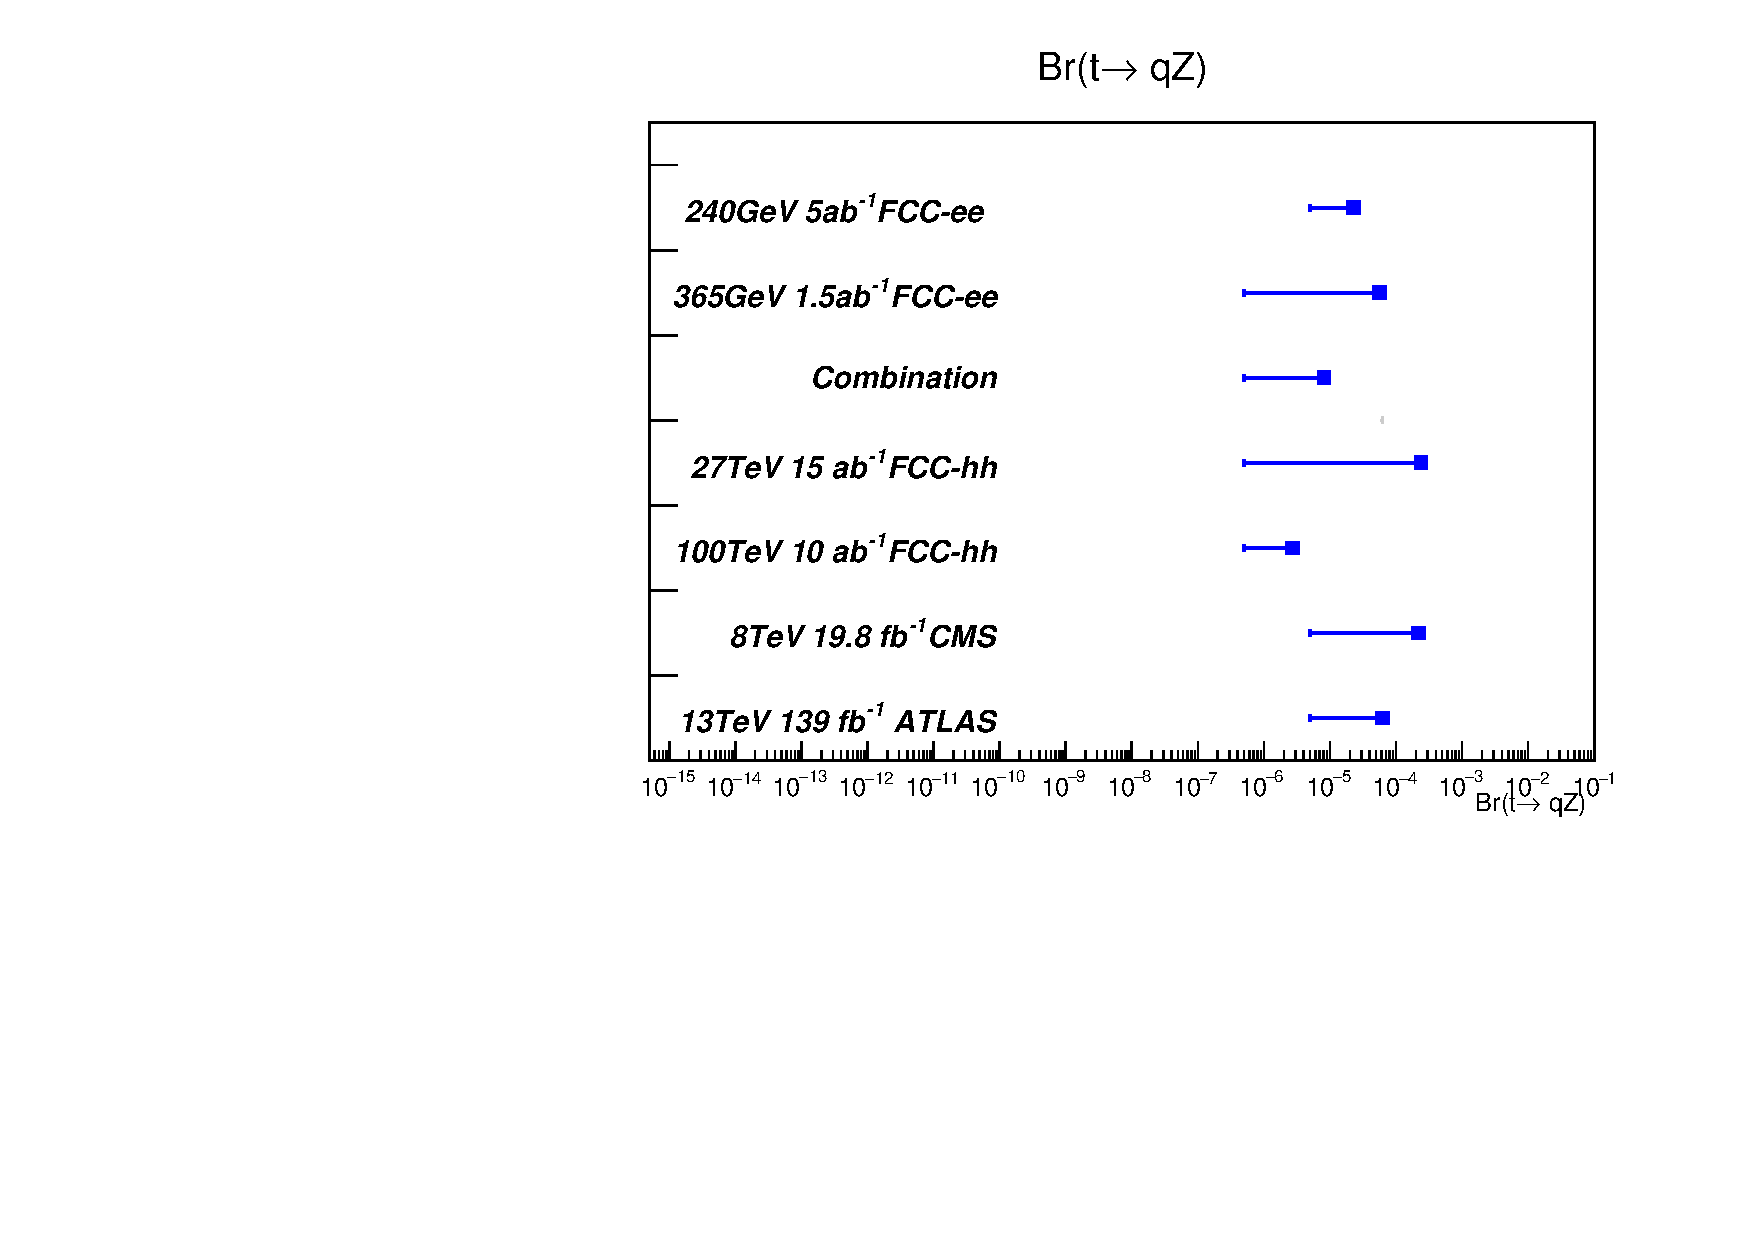
\includegraphics[width=\linewidth]{Presentation_Higgs_performance_meeting19marc_2024/tqz_compare2.pdf}
%\end{column}
%\end{columns}
%\vspace{0.25em}
%\tinyref{Local comparison figures from the analysis package. The public comparison points correspond to the public results included in the package (legacy CMS and ATLAS values) and can be refreshed for a final conference version if needed.}
%\end{column}
\end{columns}
%\refs{Internal draft note Tables VI and XI; local comparison plots included in the presentation package.}
\vspace{0.5em}
\begin{tcolorbox}[colback=white,colframe=black!30]
\small
\justifying
These limits are study-level FCC-ee projections obtained in the official framework for the benchmark luminosities: $240$\,GeV@5 $ab^{-1}$ and  $364$\,GeV@1.5 $ab^{-1}$.
\end{tcolorbox}
\end{frame}






%----------------------------------------------------------------------------------------
\begin{frame}{Main physics take-away}
\begin{columns}[T,totalwidth=\textwidth]
\begin{column}{0.50\textwidth}
\begin{itemize}
\justifying
\item FCC-ee is a precision Higgs + electroweak + top machine, not merely a single-purpose Higgs factory.
\item Top FCNC is one of the cleanest BSM probes in the top sector because the SM expectation is tiny and any visible signal would be genuinely new physics.
\item In the present FCC-ee study, single-top production driven by \(tq\gamma\) and \(tqZ\) couplings can be tested in both semileptonic and fully hadronic final states within the official analysis framework.
\item The combined semileptonic benchmark sensitivities reach the \(10^{-5}\) to \(10^{-6}\) level in branching ratio.
\end{itemize}
\end{column}
\begin{column}{0.45\textwidth}
\begin{alertblock}{Best FCCee benchmark numbers}
\centering
\(\mathrm{Br}(t\to c\gamma) < 1.99\times10^{-5}\)\\[0.4em]
\(\mathrm{Br}(t\to cZ) < 8.19\times10^{-6}\)
\end{alertblock}
\begin{alertblock}{HL-LHC (\(14\,\mathrm{TeV},\,3\,\mathrm{ab}^{-1}\))}
\centering
\begin{tabular}{@{}lc@{}}
\(\mathrm{Br}(t\to c\gamma)\) & \(7.4\times10^{-5}\) \\
\(\mathrm{Br}(t\to cZ)\)      & \(5.5\times10^{-5}\) \\
\end{tabular}
\refs{CMS-CR-2018-094; ATL-PHYS-PUB-2019-001.}
\end{alertblock}
\begin{block}{Interpretation}
\small
\justifying 
This is the type of rare-top study that demonstrates how FCC-ee precision can be turned into genuine new-physics reach. 
\end{block}
\end{column}
\end{columns}
\end{frame}






%----------------------------------------------------------------------------------------
\begin{frame}{Summary, physics message, and outlook}
\begin{itemize}
\justifying
\item We placed the FCNC study inside the broader FCC-ee programme: Higgs precision, electroweak precision, and top physics provide the natural context for rare top searches.	
\item The present analysis uses the {\color{magenta}official FCC framework}, realistic detector response, and both semileptonic and fully hadronic signal channels.
\item The clean \(e^+e^-\) environment makes FCC-ee highly competitive for probing anomalous \(tq\gamma\) and \(tqZ\) interactions through single-top production.
\item The projected sensitivities show that FCC-ee can provide a strong and complementary probe of top FCNC interactions within its wider precision programme.
\item Immediate next steps are straightforward: luminosity-scenario refresh, flavour-tagging assumptions, inclusion of systematic uncertainties, and potentially multivariate optimisation \& advanced machine-learning techniques.  
%\item FCC-ee rare-top studies are a natural and visible part of the emerging Polish FCC physics agenda.
\end{itemize}
\vspace{0.2cm}
\refs{{\color{red}Top FCNC analysis note: FCC Physics and Experiments:  https://repository.cern/records/avxy7-mtz86}.}
\end{frame}





%=====================================================
\begin{frame}%[plain,noframenumbering]
\centering

\includegraphics[width=0.85\paperwidth,height=0.85\paperheight,keepaspectratio]{Thank_You_2.jpg}
\end{frame}
%=====================================================







\end{document}



















